



%% Dokumentenklasse (Koma Script) -----------------------------------------
\documentclass[
	%draft,     % Entwurfsstadium
	final,      % fertiges Dokument
	%%%% --- Schriftgr��e ---
		10pt,
		%smallheadings,    		% kleine �berschriften
		normalheadings,   		% normale �berschriften
%		bigheadings,       		% gro�e �berschriften
	%%%% --- Sprache ---
		ngerman,				% wird an andere Pakete weitergereicht
	%%%% === Seitengr��e ===
		% letterpaper,
		% legalpaper,
		% executivepaper,
		a4paper,
		% a5paper,
		% landscap,
	%%%% === Optionen f�r den Satzspiegel ===
		%BCOR5mm,			% Zus�tzlicher Rand auf der Innenseite
		DIV20,				% Seitengr�sse (siehe Koma Skript Dokumentation !)
%		DIV11,				% Seitengr�sse (siehe Koma Skript Dokumentation !)
%		DIVcalc,				% automatische Berechnung einer guten Zeilenl�nge
		1.0headlines,			% Zeilenanzahl der Kopfzeilen
		%1.1headlines,			% Zeilenanzahl der Kopfzeilen
		%headinclude,			% Kopf einbeziehen
		headexclude,			% Kopf nicht einbeziehen
		%footinclude,			% Fuss einbeziehen
		footexclude,			% Fuss nicht einbeziehen
		mpinclude,			% Margin einbeziehen
		%mpexclude,			% Margin nicht einbeziehen
		pagesize,				% Schreibt die Papiergr�sse in die Datei. Wichtig f�r Konvertierungen
   %footskip=0pt,    % distance separation between baseline of last line of text and baseline of footer			0pt
	%%%% === Layout ===
		oneside,				% einseitiges Layout
		%twoside,				% Seitenr�nder f�r zweiseitiges Layout
		onecolumn,			% Einspaltig
		%twocolumn,			% Zweispaltig
		openany,			% Kapitel beginnen auf jeder Seite
		%openright,			% Kapitel beginnen immer auf der rechten Seite (macht nur bei 'twoside' Sinn)
		%cleardoubleplain,		% leere, linke Seite mit Seitenstil 'plain'
		%cleardoubleempty,		% leere, linke Seite mit Seitenstil 'empty'
		titlepage,				% Titel als einzelne Seite ('titlepage' Umgebung)
		%notitlepage,			% Titel in Seite integriert
	%%%% --- Absatzeinzug ---
		% Absatzabstand: Einzeilig,
			%parskip,			% Freiraum in letzter Zeile: 1em
			%parskip*,			% Freiraum in letzter Zeile: Viertel einer Zeile
			%parskip+,			% Freiraum in letzter Zeile: Drittel einer Zeile
			%parskip-,			% Freiraum in letzter Zeile: keine Vorkehrungen
		% Absatzabstand: Halbzeilig
			%halfparskip,		% Freiraum in letzter Zeile: 1em
			%halfparskip*,		% Freiraum in letzter Zeile: Viertel einer Zeile
			%halfparskip+,		% Freiraum in letzter Zeile: Drittel einer Zeile
			%halfparskip,		% Freiraum in letzter Zeile: keine Vorkehrungen
		% Absatzabstand: keiner
			parindent,			% Einger�ckt (Standard)
	%%%% --- Kolumnentitel ---
		headsepline,			% Linie unter Kolumnentitel
		%headnosepline,		% keine Linie unter Kolumnentitel
		%footsepline,			% Linie unter Fussnote
		%footnosepline,		% keine Linie unter Fussnote
	%%%% --- Kapitel ---
		%chapterprefix,		% Ausgabe von 'Kapitel:'
		nochapterprefix,		% keine Ausgabe von 'Kapitel:'
	%%%% === Verzeichnisse (TOC, LOF, LOT, BIB) ===
		%liststotoc,			% Tabellen & Abbildungsverzeichnis ins TOC
		%idxtotoc,			% Index ins TOC
		bibtotoc,			% Bibliographie ins TOC
		%bibtotocnumbered,	% Bibliographie im TOC nummeriert
		%liststotocnumbered,	% Alle Verzeichnisse im TOC nummeriert
		tocindent,			% einger�ckte Gliederung
		%tocleft,			% Tabellenartige TOC
		listsindent,			% eingereuckte LOT, LOF
		%listsleft,			% Tabellenartige LOT, LOF
		%pointednumbers,		% �berschriftnummerierung mit Punkt, siehe DUDEN !
		pointlessnumbers,		% �berschriftnummerierung ohne Punkt, siehe DUDEN !
		%openbib,			% alternative Formatierung des Literaturverzeichnisses
	%%%% === Matheformeln ===
		%leqno,				% Formelnummern links
		fleqn,				% Formeln werden linksb�ndig angezeigt
]{scrreprt}					%     Klassen: scrartcl, scrreprt, scrbook
\usepackage[per=fraction,fraction=nice]{siunitx}
\usepackage{blindtext}
% -------------------------------------------------------------------------
% Encoding der Dateien (sonst funktionieren Umlaute nicht)
		% F�r Linux							-> utf8
		% F�r MAC-OS							-> applemac
		% F�r Windows, alte Linux Distributionen		-> latin1
		% Empfohlen latin1, da einige Pakete mit utf8 Zeichen nicht funktionieren, z.B: listings, soul.
	%\usepackage[applemac]{inputenc}
	%\usepackage{lmodern,dsfont}
	\usepackage[T1]{fontenc}
	\usepackage[latin1]{inputenc}
	%\usepackage[ansinew]{inputenc}
	%\usepackage[utf8]{inputenc}
	%\usepackage{ucs}
	%\usepackage[utf8x]{inputenc}
%%% Preambel
	% ------------------------------------------------------------------------
% LaTeX - Preambel  ******************************************************
% ------------------------------------------------------------------------
% von: Matthias Pospiech
% ========================================================================

% Strukturierung dieser Praeambel:
%    1.  Pakete die vor anderen geladen werden m�ssen
%        (calc, babel, xcolor, graphicx, amsmath, pst-pdf, ragged2e, ...)
%    2.  Schriften
%    3.  Mathematik (mathtools, fixmath, onlyamsmath, braket,
%        cancel, empheq, exscale, icomma, ...)
%    4.  Tabellen (booktabs, multirow, dcolumn, tabularx, ltxtable, supertabular)
%    5.  Text
%        5.1 Auszeichnungen (ulem, soul, url)
%        5.2 Fussnoten (footmisc)
%        5.3 Verweise (varioref)
%        5.4 Listen (enumitem, paralist, declist)
%    6.  Zitieren (csquotes, jurabib, natbib)
%    7.  PDF (microtype, hyperref, backref, hypcap, pdfpages
%    8.  Graphiken (float, flafter, placeins, subfig, wrapfig,
%        floatflt, picins, psfrag, sidecap, pict2e, curve2e)
%    9.  Sonstiges (makeidx, isodate, numprint, nomencl, acronym)
%    10. Verbatim (upquote, verbatim, fancyvrb, listings, examplep)
%    11. Wissenschaft (units)
%    12. Fancy Stuff
%    13. Layout
%       13.1.  Diverse Pakete und Einstellungen (multicol, ellipsis)
%       13.2.  Zeilenabstand (setspace)
%       13.3.  Seitenlayout (typearea, geometry)
%       13.4.  Farben
%       13.5.  Aussehen der URLS
%       13.6.  Kopf und Fusszeilen (scrpage2)
%       13.7.  Fussnoten
%       13.8.  Schriften (Sections )
%       13.9.  UeberSchriften (Chapter und Sections) (titlesec, indentfirst)
%       13.10. Captions (Schrift, Aussehen)
%              (caption, subfig, capt-of, mcaption, tocloft, multitoc, minitoc)
%    14.  Auszufuehrende Befehle


% ~~~~~~~~~~~~~~~~~~~~~~~~~~~~~~~~~~~~~~~~~~~~~~~~~~~~~~~~~~~~~~~~~~~~~~~~
% Einige Pakete muessen unbedingt vor allen anderen geladen werden
% ~~~~~~~~~~~~~~~~~~~~~~~~~~~~~~~~~~~~~~~~~~~~~~~~~~~~~~~~~~~~~~~~~~~~~~~~

%%% Packages for LaTeX - programming
%
% Define commands that don't eat spaces.
\usepackage{xspace}
% IfThenElse
\usepackage{ifthen}
%%% Doc: ftp://tug.ctan.org/pub/tex-archive/macros/latex/contrib/oberdiek/ifpdf.sty
% command for testing for pdf-creation
\usepackage{ifpdf} %\ifpdf \else \fi

%%% Internal Commands: ----------------------------------------------
\makeatletter
%
\providecommand{\IfPackageLoaded}[2]{\@ifpackageloaded{#1}{#2}{}}
\providecommand{\IfPackageNotLoaded}[2]{\@ifpackageloaded{#1}{}{#2}}
\providecommand{\IfElsePackageLoaded}[3]{\@ifpackageloaded{#1}{#2}{#3}}
%
\newboolean{chapteravailable}%
\setboolean{chapteravailable}{false}%

\ifcsname chapter\endcsname
  \setboolean{chapteravailable}{true}%
\else
  \setboolean{chapteravailable}{false}%
\fi


\providecommand{\IfChapterDefined}[1]{\ifthenelse{\boolean{chapteravailable}}{#1}{}}%
\providecommand{\IfElseChapterDefined}[2]{\ifthenelse{\boolean{chapteravailable}}{#1}{#2}}%

\providecommand{\IfDefined}[2]{%
\ifcsname #1\endcsname
   #2 %
\else
     % do nothing
\fi
}

\providecommand{\IfElseDefined}[3]{%
\ifcsname #1\endcsname
   #2 %
\else
   #3 %
\fi
}

\providecommand{\IfElseUnDefined}[3]{%
\ifcsname #1\endcsname
   #3 %
\else
   #2 %
\fi
}


%
% Check for 'draft' mode - commands.
\newcommand{\IfNotDraft}[1]{\ifx\@draft\@undefined #1 \fi}
\newcommand{\IfNotDraftElse}[2]{\ifx\@draft\@undefined #1 \else #2 \fi}
\newcommand{\IfDraft}[1]{\ifx\@draft\@undefined \else #1 \fi}
%

% Definde frontmatter, mainmatter and backmatter if not defined
\@ifundefined{frontmatter}{%
   \newcommand{\frontmatter}{%
      %In Roemischen Buchstaben nummerieren (i, ii, iii)
      \pagenumbering{roman}
   }
}{}
\@ifundefined{mainmatter}{%
   % scrpage2 benoetigt den folgenden switch
   % wenn \mainmatter definiert ist.
   \newif\if@mainmatter\@mainmattertrue
   \newcommand{\mainmatter}{%
      % -- Seitennummerierung auf Arabische Zahlen zuruecksetzen (1,2,3)
      \pagenumbering{arabic}%
      \setcounter{page}{1}%
   }
}{}
\@ifundefined{backmatter}{%
   \newcommand{\backmatter}{
      %In Roemischen Buchstaben nummerieren (i, ii, iii)
      \pagenumbering{roman}
   }
}{}

% Pakete speichern die spaeter geladen werden sollen
\newcommand{\LoadPackagesNow}{}
\newcommand{\LoadPackageLater}[1]{%
   \g@addto@macro{\LoadPackagesNow}{%
      \usepackage{#1}%
   }%
}



\makeatother
%%% ----------------------------------------------------------------
%
%%% Doc: www.cs.brown.edu/system/software/latex/doc/calc.pdf
% Calculation with LaTeX
\usepackage{calc}

%%% Doc: ftp://tug.ctan.org/pub/tex-archive/macros/latex/required/babel/babel.pdf
% Languagesetting
\usepackage[
%	german,
	ngerman,
%	english,
%	frensh,
]{babel}

%%% Doc: ftp://tug.ctan.org/pub/tex-archive/macros/latex/contrib/xcolor/xcolor.pdf
% Farben
% Incompatible: Do not load when using pstricks !
\usepackage[
	table % Load for using rowcolors command in tables
]{xcolor}


%%% Doc: ftp://tug.ctan.org/pub/tex-archive/macros/latex/required/graphics/grfguide.pdf
% Bilder
\usepackage[%
	%final,
	%draft % do not include images (faster)
]{graphicx}

%%% Doc: ftp://tug.ctan.org/pub/tex-archive/macros/latex/contrib/oberdiek/epstopdf.pdf
%% If an eps image is detected, epstopdf is automatically called to convert it to pdf format.
%% Requires: graphicx loaded
\usepackage{epstopdf}


%%% Doc: ftp://tug.ctan.org/pub/tex-archive/macros/latex/required/amslatex/math/amsldoc.pdf
% Amsmath - Mathematik Basispaket
%
% fuer pst-pdf displaymath Modus vor pst-pdf benoetigt.
\usepackage[
   %centertags, % (default) center tags vertically
   tbtags,    % 'Top-or-bottom tags': For a split equation, place equation numbers level
               % with the last (resp. first) line, if numbers are on the right (resp. left).
   sumlimits,  %(default) Place the subscripts and superscripts of summation
               % symbols above and below
   %nosumlimits, % Always place the subscripts and superscripts of summation-type
               % symbols to the side, even in displayed equations.
   intlimits,  % Like sumlimits, but for integral symbols.
   %nointlimits, % (default) Opposite of intlimits.
   namelimits, % (default) Like sumlimits, but for certain 'operator names' such as
               % det, inf, lim, max, min, that traditionally have subscripts placed underneath
               % when they occur in a displayed equation.
   %nonamelimits, % Opposite of namelimits.
   %leqno,     % Place equation numbers on the left.
   %reqno,     % Place equation numbers on the right.
   %fleqn,     % Position equations at a fixed indent from the left margin rather than
               % centered in the text column.
]{amsmath} %
% eqnarray nicht zusammen mit amsmath benutzen, siehe l2tabu.pdf f�r Hintergruende.

%%% Doc: http://www.ctan.org/tex-archive/macros/latex/contrib/pst-pdf/pst-pdf-DE.pdf
% Used to automatically integrate eps graphics in an pdf document using pdflatex.
% Requires ps4pdf macro !!!
% Download macro from http://www.ctan.org/tex-archive/macros/latex/contrib/pst-pdf/scripts/
%
%\usepackage[%
%   %active,       % Aktiviert den Extraktionsmodus (DVI-Ausgabe). Die explizite Angabe ist
%                  % normalerweise unn�tig (Standard im LATEX-Modus).
%   %inactive,     % Das Paket wird deaktiviert, Zu�tzlich werden die Pakete pstricks und
%                  % graphicx geladen
%   nopstricks,    % Das Paket pstricks wird nicht geladen.
%   %draft,        % Im pdfLATEX-Modus werden aus der Containerdatei eingef�gte Grafiken nur
%                  % als Rahmen dargestellt.
%   %final,        % Im pdfLATEX-Modus werden aus der Containerdatei eingef�gte Grafiken
%                  % vollst�ndig dargestellt (Standard).
%   %tightpage,    % Die Abmessung Grafiken in der Containerdatei entsprechen denen der
%                  % zugeh�rigen TEX-Boxen (Standard).
%   %notightpage,  % die Grafiken in der Containerdatei nehmen
%                  % mindestens die Gr��e des gesamten Blattes einnehmen.
%   %displaymath,  % Es werden zus�tzlich die mathematischen Umgebungen displaymath,
%                  % eqnarray und $$ extrahiert und im pdf-Modus als Grafik eingef�gt.
%]{pst-pdf}
%
% Notwendiger Bugfix f�r natbib Paket bei Benutzung von pst-pdf (Version <= v1.1o)
\IfPackageLoaded{pst-pdf}{
   \providecommand\makeindex{}
   \providecommand\makeglossary{}
}{}


%% Doc: ftp://tug.ctan.org/pub/tex-archive/graphics/pstricks/README
% load before graphicx
% \usepackage{pstricks}
% \usepackage{pst-plot, pst-node, pst-coil, pst-eps}

% This package implements a workaround for the LaTeX bug that marginpars
% sometimes appear on the wrong margin.
% \usepackage{mparhack}
% in some case this causes an error in the index together with package pdfpages
% the reason is unkown. Therefore I recommend to use the margins of marginnote

%% Doc: ftp://tug.ctan.org/pub/tex-archive/macros/latex/contrib/marginnote/marginnote.pdf
% Summary description: marginnote allows margin note, where \marginpar fails
\usepackage{marginnote}


%% Doc: (inside relsize.sty )
%% ftp://tug.ctan.org/pub/tex-archive/macros/latex/contrib/misc/relsize.sty
%  Set the font size relative to the current font size
\usepackage{relsize}

%% Doc: ftp://tug.ctan.org/pub/tex-archive/macros/latex/contrib/ms/ragged2e.pdf
% Besserer Flatternsatz (Linksbuendig, statt Blocksatz)
\usepackage{ragged2e}

% ~~~~~~~~~~~~~~~~~~~~~~~~~~~~~~~~~~~~~~~~~~~~~~~~~~~~~~~~~~~~~~~~~~~~~~~~
% Fonts Fonts Fonts
% ~~~~~~~~~~~~~~~~~~~~~~~~~~~~~~~~~~~~~~~~~~~~~~~~~~~~~~~~~~~~~~~~~~~~~~~~

\usepackage[T1]{fontenc} % T1 Schrift Encoding
\usepackage{textcomp}	 % Zusatzliche Symbole (Text Companion font extension)

%%% Schriften werden in Fonts.tex geladen
% ~~~~~~~~~~~~~~~~~~~~~~~~~~~~~~~~~~~~~~~~~~~~~~~~~~~~~~~~~~~~~~~~~~~~~~~~
% Fonts Fonts Fonts
% ~~~~~~~~~~~~~~~~~~~~~~~~~~~~~~~~~~~~~~~~~~~~~~~~~~~~~~~~~~~~~~~~~~~~~~~~

% Alle Schriften die hier angegeben sind sehen im PDF richtig aus.
% Die LaTeX Standardschrift ist die Latin Modern (lmodern Paket).
% If Latin Modern is not available for your distribution you must install the
% package cm-super instead. Otherwise your fonts will look horrible in the PDF

% DO NOT LOAD ae Package for the font !

%% ==== Zusammengesetzte Schriften  (Sans + Serif) =======================

%% - Latin Modern
\usepackage{lmodern}
%% -------------------
%
%% - Times, Helvetica, Courier (Word Standard...)
%\usepackage{mathptmx}
%\usepackage[scaled=.90]{helvet}
%\usepackage{courier}
%% -------------------
%%
%% - Palantino , Helvetica, Courier
%\usepackage{mathpazo}
%\usepackage[scaled=.95]{helvet}
%\usepackage{courier}
%% -------------------
%
%% - Bera Schriften
%\usepackage{bera}
%% -------------------
%
%% - Charter, Bera Sans
%\usepackage{charter}\linespread{1.05}
%\renewcommand{\sfdefault}{fvs}

%% ===== Serifen =========================================================

%\usepackage{mathpazo}                 %% --- Palantino
%\usepackage{charter}\linespread{1.05} %% --- Charter
%\usepackage{bookman}                  %% --- Bookman (laedt Avant Garde !!)
%\usepackage{newcent}                  %% --- New Century Schoolbook (laedt Avant Garde !!)

%\usepackage[%                         %% --- Fourier
%   upright,     % Math fonts are upright
%   expert,      % Only for EXPERT Fonts!
%   oldstyle,    % Only for EXPERT Fonts!
%   fulloldstyle % Only for EXPERT Fonts!
%]{fourier} %



%% ===== Sans Serif ======================================================

%\usepackage[scaled=.95]{helvet}        %% --- Helvetica
%\usepackage{cmbright}                  %% --- CM-Bright (eigntlich eine Familie)
%\usepackage{tpslifonts}                %% --- tpslifonts % Font for Slides
%\usepackage{avantgar}                  %% --- Avantgarde

%%%% =========== Italics ================

%\usepackage{chancery}                  %% --- Zapf Chancery

%%%% =========== Typewriter =============

%\usepackage{courier}                   %% --- Courier
%\renewcommand{\ttdefault}{cmtl}        %% --- CmBright Typewriter Font
%\usepackage[%                          %% --- Luxi Mono (Typewriter)
%   scaled=0.9
%]{luximono}



%%%% =========== Mathe ================

%% Recommanded to use with fonts: Aldus, Garamond, Melior, Sabon
%\usepackage[                           %% --- EulerVM (MATH)
%   small,       %for smaller Fonts
%  euler-digits % digits in euler fonts style
%]{eulervm}

% \usepackage[
% %   utopia,
% %   garamond,
%    charter
% ]{mathdesign}

%%%% (((( !!! kommerzielle Schriften !!! )))))))))))))))))))))))))))))))))))))))))))))))))))

%% ===== Serifen (kommerzielle Schriften ) ================================

%% --- Adobe Aldus
%\renewcommand{\rmdefault}{pasx}
%\renewcommand{\rmdefault}{pasj} %%oldstyle digits
% math recommended: \usepackage[small]{eulervm}

%% --- Adobe Garamond
%\usepackage[%
%   osf,        % oldstyle digits
%   scaled=1.05 %appropriate in many cases
%]{xagaramon}
% math recommended: \usepackage{eulervm}

%% --- Adobe Stempel Garamond
%\renewcommand{\rmdefault}{pegx}
%\renewcommand{\rmdefault}{pegj} %%oldstyle digits

%% --- Adobe Melior
%\renewcommand{\rmdefault}{pml}
% math recommended: %\usepackage{eulervm}

%% --- Adobe Minion
%\renewcommand{\rmdefault}{pmnx}
%\renewcommand{\rmdefault}{pmnj} %oldstyle digits
% math recommended: \usepackage[small]{eulervm} or \usepackage{mathpmnt} % commercial

%% --- Adobe Sabon
%\renewcommand{\rmdefault}{psbx}
%\renewcommand{\rmdefault}{psbj} %oldstyle digits
% math recommended: \usepackage{eulervm}

%% --- Adobe Times
% math recommended: \usepackage{mathptmx} % load first !
%\renewcommand{\rmdefault}{ptmx}
%\renewcommand{\rmdefault}{ptmj} %oldstyle digits

%% --- Linotype ITC Charter
%\renewcommand{\rmdefault}{lch}

%% --- Linotype Meridien
%\renewcommand{\rmdefault}{lmd}

%%% ===== Sans Serif (kommerzielle Schriften) ============================

%% --- Adobe Frutiger
%\usepackage[
%   scaled=0.90
%]{frutiger}

%% --- Adobe Futura (=Linotype FuturaLT) : Sans Serif
%\usepackage[
%   scaled=0.94  % appropriate in many cases
%]{futura}

%% --- Adobe Gill Sans : Sans Serif
%\usepackage{gillsans}

%% -- Adobe Myriad  : Sans Serif
%\renewcommand{\sfdefault}{pmy}
%\renewcommand{\sfdefault}{pmyc} %% condensed Font

%% --- Syntax : sans serif font
%\usepackage[
%   scaled
%]{asyntax}

%% --- Adobe Optima : Semi Sans Serif
%\usepackage[
%   medium %darker medium weight fonts
%]{optima}

%% --- Linotype ITC Officina Sans
%\renewcommand{\sfdefault}{lo9}





% ~~~~~~~~~~~~~~~~~~~~~~~~~~~~~~~~~~~~~~~~~~~~~~~~~~~~~~~~~~~~~~~~~~~~~~~~
% Math Packages
% ~~~~~~~~~~~~~~~~~~~~~~~~~~~~~~~~~~~~~~~~~~~~~~~~~~~~~~~~~~~~~~~~~~~~~~~~

% *** Mathematik **************************************
%
% amsmath schon vorher geladen da es vor pst-pdf geladen werden muss


%%% Doc: ftp://tug.ctan.org/pub/tex-archive/macros/latex/contrib/mh/doc/mathtools.pdf
% Erweitert amsmath und behebt einige Bugs
\usepackage[fixamsmath,disallowspaces]{mathtools}

%%% Doc: http://www.ctan.org/info?id=fixmath
% LaTeX's default style of typesetting mathematics does not comply
% with the International Standards ISO31-0:1992 to ISO31-13:1992
% which indicate that uppercase Greek letters always be typset
% upright, as opposed to italic (even though they usually
% represent variables) and allow for typsetting of variables in a
% boldface italic style (even though the required fonts are
% available). This package ensures that uppercase Greek be typeset
% in italic style, that upright $\Delta$ and $\Omega$ symbols are
% available through the commands \upDelta and \upOmega; and
% provides a new math alphabet \mathbold for boldface
% italic letters, including Greek.
\usepackage{fixmath}

%%% Doc: ftp://tug.ctan.org/pub/tex-archive/macros/latex/contrib/onlyamsmath/onlyamsmath.dvi
% Warnt bei Benutzung von Befehlen die mit amsmath inkompatibel sind.
\usepackage[
	all,
	warning
]{onlyamsmath}


%------------------------------------------------------

% -- Vektor fett darstellen -----------------
% \let\oldvec\vec
% \def\vec#1{{\boldsymbol{#1}}} %Fetter Vektor
% \newcommand{\ve}{\vec} %
% -------------------------------------------


%%% Doc: ftp://tug.ctan.org/pub/tex-archive/macros/latex/contrib/misc/braket.sty
\usepackage{braket}  % Quantenmechanik Bracket Schreibweise

%%% Doc: ftp://tug.ctan.org/pub/tex-archive/macros/latex/contrib/misc/cancel.sty
\usepackage{cancel}  % Durchstreichen

%%% Doc: ftp://tug.ctan.org/pub/tex-archive/macros/latex/contrib/mh/doc/empheq.pdf
\usepackage{empheq}  % Hervorheben

%%% Doc: ftp://tug.ctan.org/pub/tex-archive/info/math/voss/mathmode/Mathmode.pdf
%\usepackage{exscale} % Skaliert Mathe-Modus Ausgaben in allen Umgebungen richtig.

%%% Doc: ftp://tug.ctan.org/pub/tex-archive/macros/latex/contrib/was/icomma.dtx
% Erlaubt die Benutzung von Kommas im Mathematikmodus
\usepackage{icomma}


%%% Doc: http://www.ctex.org/documents/packages/special/units.pdf
% \usepackage[nice]{nicefrac}

%%% Tauschen von Epsilon und andere:
% \let\ORGvarrho=\varrho
% \let\varrho=\rho
% \let\rho=\ORGvarrho
%
\let\ORGvarepsilon=\varepsilon
\let\varepsilon=\epsilon
\let\epsilon=\ORGvarepsilon
%
% \let\ORGvartheta=\vartheta
% \let\vartheta=\theta
% \let\theta=\ORGvartheta
%
% \let\ORGvarphi=\varphi
% \let\varphi=\phi
% \let\phi=\ORGvarphi

% ~~~~~~~~~~~~~~~~~~~~~~~~~~~~~~~~~~~~~~~~~~~~~~~~~~~~~~~~~~~~~~~~~~~~~~~~
% Symbole
% ~~~~~~~~~~~~~~~~~~~~~~~~~~~~~~~~~~~~~~~~~~~~~~~~~~~~~~~~~~~~~~~~~~~~~~~~
%
%%% General Doc: http://www.ctan.org/tex-archive/info/symbols/comprehensive/symbols-a4.pdf
%
%% Symbole f�r Mathematiksatz
\usepackage{mathrsfs} %% Schreibschriftbuchstaben f�r den Mathematiksatz (nur Gro�buchstaben)
\usepackage{dsfont}   %% Double Stroke Fonts
\usepackage[mathcal]{euscript} %% adds euler mathcal font
\usepackage{amssymb}
\usepackage[Symbolsmallscale]{upgreek} % upright symbols from euler package [Euler] or Adobe Symbols [Symbol]
\usepackage[upmu]{gensymb}             % Option upmu

%% Allgemeine Symbole
\usepackage{wasysym}  %% Doc: http://www.ctan.org/tex-archive/macros/latex/contrib/wasysym/wasysym.pdf
%\usepackage{marvosym} %% Symbole aus der marvosym Schrift
\usepackage{pifont}   %% ZapfDingbats


% ~~~~~~~~~~~~~~~~~~~~~~~~~~~~~~~~~~~~~~~~~~~~~~~~~~~~~~~~~~~~~~~~~~~~~~~~
% Tables (Tabular)
% ~~~~~~~~~~~~~~~~~~~~~~~~~~~~~~~~~~~~~~~~~~~~~~~~~~~~~~~~~~~~~~~~~~~~~~~~

% Basispaket fuer alle Tabellenfunktionen
% -> wird automatisch durch andere Pakete geladen
% \usepackage{array}
%
% bessere Abstaende innerhalb der Tabelle (Layout))
% -------------------------------------------------
%%% Doc: ftp://tug.ctan.org/pub/tex-archive/macros/latex/contrib/booktabs/booktabs.pdf
\usepackage{booktabs}
%
% Farbige Tabellen
% ----------------
% Das Paket colortbl wird inzwischen automatisch durch xcolor geladen
%
% Erweiterte Funktionen innerhalb von Tabellen
% --------------------------------------------
%%% Doc: ftp://tug.ctan.org/pub/tex-archive/macros/latex/contrib/multirow/multirow.sty
\usepackage{multirow} % Mehrfachspalten
%
%%% Doc: Documentation inside dtx Package
\usepackage{dcolumn}  % Ausrichtung an Komma oder Punkt

%%% Neue Tabellen-Umgebungen:
% ---------------------------
% Spalten automatischer Breite:
%%% Doc: Documentation inside dtx Package
% \usepackage{tabularx}
% -> nach hyperref Laden
% -> wird von ltxtable geladen
% \LoadPackageLater{tabularx}


% Tabellen ueber mehere Seiten
% ----------------------------
%%% Doc: ftp://tug.ctan.org/pub/tex-archive/macros/latex/contrib/carlisle/ltxtable.pdf
% \usepackage{ltxtable} % Longtable + tabularx
                        % (multi-page tables) + (auto-sized columns in a fixed width table)
% -> nach hyperref laden
\LoadPackageLater{ltxtable}


%%% Doc: ftp://tug.ctan.org/pub/tex-archive/macros/latex/contrib/supertabular/supertabular.pdf
%\usepackage{supertabular}


% ~~~~~~~~~~~~~~~~~~~~~~~~~~~~~~~~~~~~~~~~~~~~~~~~~~~~~~~~~~~~~~~~~~~~~~~~
% text related packages
% ~~~~~~~~~~~~~~~~~~~~~~~~~~~~~~~~~~~~~~~~~~~~~~~~~~~~~~~~~~~~~~~~~~~~~~~~

%%% Textverzierungen/Auszeichnungen ======================================
%
%%% Doc: ftp://tug.ctan.org/pub/tex-archive/macros/latex/contrib/misc/ulem.sty
\usepackage[normalem]{ulem}      % Zum Unterstreichen
%%% Doc: ftp://tug.ctan.org/pub/tex-archive/macros/latex/contrib/soul/soul.pdf
\usepackage{soul}		            % Unterstreichen, Sperren
%%% Doc: ftp://tug.ctan.org/pub/tex-archive/macros/latex/contrib/misc/url.sty
\usepackage{url} % Setzen von URLs. In Verbindung mit hyperref sind diese auch aktive Links.

%%% Fussnoten/Endnoten ===================================================
%
%%% Doc: ftp://tug.ctan.org/pub/tex-archive/macros/latex/contrib/footmisc/footmisc.pdf
%
\usepackage[
   bottom,      % Footnotes appear always on bottom. This is necessary
                % especially when floats are used
   stable,      % Make footnotes stable in section titles
   perpage,     % Reset on each page
   %para,       % Place footnotes side by side of in one paragraph.
   %side,       % Place footnotes in the margin
   ragged,      % Use RaggedRight
   %norule,     % suppress rule above footnotes
   multiple,    % rearrange multiple footnotes intelligent in the text.
   %symbol,     % use symbols instead of numbers
]{footmisc}

%% Einruecken der Fussnote einstellen
%\setlength\footnotemargin{10pt}

%--- footnote counter documentweit durchlaufend ------------------------------
%\usepackage{chngcntr}
%\counterwithout{footnote}{chapter}
%-----------------------------------------------------------------------------

%%% Doc: ftp://tug.ctan.org/pub/tex-archive/macros/latex/contrib/misc/endnotes.sty
%\usepackage{endnotes}
% From the Documentation:
% To turn all the footnotes in your documents into endnotes, say
%
%     \let\footnote=\endnote
%
%  in your preamble, and then add something like
%
%     \newpage
%     \begingroup
%     \parindent 0pt
%     \parskip 2ex
%     \def\enotesize{\normalsize}
%     \theendnotes
%     \endgroup
%
% as the last thing in your document.  (But \theendnotes all
% by itself will work.)

%%% Verweise =============================================================
%
%%% Doc: Documentation inside dtx File
\usepackage[ngerman]{varioref} % Intelligente Querverweise

%%% Listen ===============================================================
%
%
%%% Doc: ftp://tug.ctan.org/pub/tex-archive/macros/latex/contrib/paralist/paralist.pdf
% \usepackage{paralist}
%
%%% Doc: ftp://tug.ctan.org/pub/tex-archive/macros/latex/contrib/enumitem/enumitem.pdf
% Better than 'paralist' and 'enumerate' because it uses a keyvalue interface !
% Do not load together with enumerate.
\IfPackageNotLoaded{enumerate}{
	\usepackage{enumitem}
}
%
%%% Doc: ftp://tug.ctan.org/pub/tex-archive/macros/latex/contrib/ncctools/doc/desclist.pdf
% Improved description environment
%\usepackage{declist}


% ~~~~~~~~~~~~~~~~~~~~~~~~~~~~~~~~~~~~~~~~~~~~~~~~~~~~~~~~~~~~~~~~~~~~~~~~
% Pakete zum Zitieren
% ~~~~~~~~~~~~~~~~~~~~~~~~~~~~~~~~~~~~~~~~~~~~~~~~~~~~~~~~~~~~~~~~~~~~~~~~

% Quotes =================================================================
%% Doc: ftp://tug.ctan.org/pub/tex-archive/macros/latex/contrib/csquotes/csquotes.pdf
% Advanced features for clever quotations
\usepackage[%
   babel,            % the style of all quotation marks will be adapted
                     % to the document language as chosen by 'babel'
   german=quotes,		% Styles of quotes in each language
   english=british,
   french=guillemets
]{csquotes}

% All facilities which take a 'cite' argument will not insert
% it directly. They pass it to an auxiliary command called \mkcitation
% which  may be redefined to format the citation.
\renewcommand*{\mkcitation}[1]{{\,}#1}
\renewcommand*{\mkccitation}[1]{ #1}

\SetBlockThreshold{2} % Anzahl von Zeilen

\newenvironment{myquote}%
	{\begin{quote}\small}%
	{\end{quote}}%
\SetBlockEnvironment{myquote}
%\SetCiteCommand{} % Changes citation command


% Zitate =================================================================
%
% Reference by number
% \makeatletter
% \renewcommand\@biblabel[1]{#1.}
% \makeatother

% -------- Reference by author -------------------------------------------

% Doc: http://www.berger-on.net/jurabib/
% \usepackage{jurabib}
% \jurabibsetup{
%    authorformat={
%       %abbrv,%  First names will be abbreviated
%       %allreversed,% Names will be printed reversed ('first surname' in text and bibliography)
%       %citationreversed,% Names will be printed reversed ('first surname' only in text)
%       and,% Author separation with ',' and ', and' instead of the default slashes
%       %dynamic,% Font of author depends on existence of coauthor
%       %firstnotreversed, %All author names (except the first) will be printed reversed (in text only)
%       %indexed,% All author names are indexed separately (makeidx or index have to be loaded appropriately)
%       %italic,% Author will appear in italics
%       %reducedifibidem,%  Author names are reduced to the surname for subsequent
%       %citations,% (for the ibidem=name options)
%       smallcaps,% Author will appear in small caps
%       year,% Emulates author-year citations
%    },
%    bibformat={
%       %compress,% Reduces the vertical space between the items in the bibliography
%       %ibidem,%  Replaces repeated authors in the bibliography
%       %ibidemalt,% Special format for German law students
%       %nohang,% No hanging indent for bibliography
%       numbered,% Numbered items in bibliography
%       %raggedright,% Flushleft for bibliography
%       %tabular,% Tabular-like bibliography format
%    },
%    titleformat={
%       all,% Prints out all titles, doesn't care about multiple works
%       %colonsep,% Separation between author and title with colon
%       comma,% Separation between author and title with comma
%       italic,% Title will appear in italics
%    },
%    %biblikecite=true,% Formatting of bibliography follows formatting of citations (as far as possible)
%    %coauthorformat={
%    %  normal,% No special format for coauthors
%    %  %italic,% Coauthor will appear in italics
%    %},
%    %colastsep=divis,% Coauthor after author, separation with divis, Standard is a slash
%    %cofirstsep={
%    %% in,% Author after coauthor, separation with 'in'
%    %  comma,% Author after coauthor, separation with comma
%    %},
%    commabeforerest,  % Nach allen Angaben und vor den zusaetzlichen
%                      % (z.B. Seitenanzahl) wird ein Komma gesetzt
%    citefull={
%       %all,% All citations are full citations
%       first,% First citation is printed full
%       %chapter,% citefull=first, resetted each chapter (book and report classes)
%       %section,% citefull=first, resetted each section (article classes)
%    },
%    %chicago=true, %chicago-like format of citation and bibliography
%    %oxford=true, %Emulates oxford-like format of citation and bibliography
%    %crossref={
%    %  dynamic,% Long crossref's if they are used first time, shorter for all further citations
%    %  long,% Always long crossref's
%    %  short,% Always short crossref's (short as possible, longer if citations are ambiguous)
%    %},
%    %edby=true,% Switches from '(ed.)' to 'edited by' for incollections
%    %endnote=true,% The note field is printed at the end of the entry, after the closing period
%    %footnotes=marginal,% Another footnote format
%    %human=true, % Common humanities option, make authorformat=and the default
%    %howcited={
%    %  all,% The howcited remark is printed for all entries
%    %  compare,% The howcited remark is printed for works, where title and shorttitle differ
%    %  normal,% The howcited remark is printed for entries containing a non-empty howcited field
%    %  multiple,%  The howcited remark is printed if more than one work of the author is cited
%    %},
%    ibidem={
%       %name,% Ibidem with authors name
%       %name&title,% Ibidem with authors name and title
%       %nostrict,% Ibidem is allowed for every footnote
%       strict,% Ibidem is not allowed for first footnote on each page
%       %strictdoublepage,% Ibidem is not allowed for first footnote on left (even) pages
%    },
%    idem={
%       %nostrict,% Idem is allowed for every footnote
%       strict,% Idem is not allowed for first footnote on each page
%       %strictdoublepage,%  Idem is not allowed for first footnote on left (even) pages
%    },
%    %lookat=true,% Enables crossref to full (first) footnote citation
%    %natoptargorder=true,% Reversed optional arguments
%    %opcit={
%    %  true,% Enables op. cit. for already cited, but not subsequent works
%    %  chapter,% Resets opcit each chapter (book and report classes)
%    %  section,% Resets opcit each section (article classes)
%    %},
%    pages={
%       %always,%  Page(ranges)s given via the pages-field are always printed in the citation
%       format,%  Pages given via the optional argument and page(ranges)s given via the pages-field are formatted automatically
%       %test,% Page(ranges)s given via the pages-field are printed in the citation, if no pages are given by the optional argument
%    },
%    %see=true,% The second optional argument can be used to add sequences like 'see' before the citation
%    %superscriptedition={
%    %  all,% Superscripted edition number for all citations
%    %  bib,% Superscripted edition number for the bibliography
%    %  commented,% Superscripted edition number only for type @COMMENTED
%    %  switch,%  Superscripted edition number for works with field ssedition=1
%    %},
%    super, % alle \cite werden zu footcite
% }
%
% \bibliographystyle{jurabib} %
% %\bibliographystyle{jureco}
% %\bibliographystyle{jurunsrt}
% %\bibliographystyle{jox}
%
% \renewcommand{\biblnfont}{\bfseries\scshape\RaggedRight} % Autoren
% \renewcommand{\bibfnfont}{} % Autoren Vornamen
% \renewcommand{\bibelnfont}{\normalfont} % Herausgeber
% \renewcommand{\bibefnfont}{\normalfont} % Herausgeber Vornamen
% % Anpassung der Titel von Buechern
% \renewcommand{\bibtfont}{\normalfont\textit} % Titel
% % % Modifizierung des Zeitschriftentitels bei Artikeln.
% \renewcommand{\bibjtfont}{\normalfont}
% % % Titel eines Artikels, eines Beitrages in einem Sammelwerk oder aehnliches zu formatieren.
% \renewcommand{\bibapifont}{\normalfont\textit} % Periodical-Titel
% % % Aussehen des series Feldes bestimmen
% \renewcommand{\bibsnfont}{\textbf}
% %
% \renewcommand{\biburlprefix}{Webseite:{ }}
% \renewcommand{\biburlsuffix}{}
%
% % Ausgabe des Jahres
% \renewcommand{\jbcitationyearformat}[1]{(#1)}
%
% \renewcommand{\bibleftcolumnadjust}{\RaggedRight}
% \renewcommand{\bibrightcolumnadjust}{\RaggedRight}
% %
% -------- Reference by number (author) ----------------------------------

% %%% Doc: ftp://tug.ctan.org/pub/tex-archive/macros/latex/contrib/natbib/natbib.pdf
\usepackage[%
	%round,	%(default) for round parentheses;
	square,	% for square brackets;
	%curly,	% for curly braces;
	%angle,	% for angle brackets;
	%colon,	% (default) to separate multiple citations with colons;
	comma,	% to use commas as separaters;
	%authoryear,% (default) for author-year citations;
	numbers,	% for numerical citations;
	%super,	% for superscripted numerical citations, as in Nature;
	sort,		% orders multiple citations into the sequence in which they appear in the list of references;
	sort&compress,    % as sort but in addition multiple numerical citations
                   % are compressed if possible (as 3-6, 15);
	%longnamesfirst,  % makes the first citation of any reference the equivalent of
                   % the starred variant (full author list) and subsequent citations
                   %normal (abbreviated list);
	%sectionbib,      % redefines \thebibliography to issue \section* instead of \chapter*;
                   % valid only for classes with a \chapter command;
                   % to be used with the chapterbib package;
	%nonamebreak,     % keeps all the authors names in a citation on one line;
                   %causes overfull hboxes but helps with some hyperref problems.
]{natbib}

%%% Bibliography styles with natbib support
%\bibliographystyle{plainnat} % Numeric Labels, alphabatical order
%\bibliographystyle{abbrvnat} % same as plain, but shorter names
%\bibliographystyle{unsrtnat} % same as plain, but appeariance in order of citation
%\bibliographystyle{alpha}    % labels are formed by author and year

%%% Bibliography styles according to DIN
%%% get from: http://www.ctan.org/tex-archive/biblio/bibtex/contrib/german/din1505/
%\bibliographystyle{alphadin}
%\bibliographystyle{abbrvdin}
%\bibliographystyle{plaindin}
%\bibliographystyle{unsrtdin}
%\bibliographystyle{bib/bst/alphadin-mod} % Modifiziert: Kleinere Abstaende vor ";" und kein "+" bei etal.

%%% Bibliography styles created with custombib
%%% Doc: ftp://tug.ctan.org/pub/tex-archive/macros/latex/contrib/custom-bib/makebst.pdf
\bibliographystyle{bib/bst/AlphaDINFirstName}

% other BibTeX styles: http://www.cs.stir.ac.uk/~kjt/software/latex/showbst.html

% ~~~~~~~~~~~~~~~~~~~~~~~~~~~~~~~~~~~~~~~~~~~~~~~~~~~~~~~~~~~~~~~~~~~~~~~~
% PDF related packages
% ~~~~~~~~~~~~~~~~~~~~~~~~~~~~~~~~~~~~~~~~~~~~~~~~~~~~~~~~~~~~~~~~~~~~~~~~

%%% Doc: ftp://tug.ctan.org/pub/tex-archive/macros/latex/contrib/microtype/microtype.pdf
% Optischer Randausgleich mit pdfTeX
\ifpdf
\usepackage[%
	expansion=true, % better typography, but with much larger PDF file.
	protrusion=true
]{microtype}
\fi


%% Use only instead of hyperref !
% \usepackage[%
%    %ref,     % verweist auf Abschnitte
%    pageref, % verweist auf Seiten
% ]{backref} % Links in BiB back to Citation page/section (can be loaded by hyperref too)


%%% Doc: ftp://tug.ctan.org/pub/tex-archive/macros/latex/contrib/hyperref/doc/manual.pdf
\usepackage[
   % Farben fuer die Links
   colorlinks=true,         % Links erhalten Farben statt Kaeten
   urlcolor=pdfurlcolor,    % \href{...}{...} external (URL)
   filecolor=pdffilecolor,  % \href{...} local file
   linkcolor=pdflinkcolor,  %\ref{...} and \pageref{...}
   % Links
   raiselinks=true,			 % calculate real height of the link
   breaklinks,              % Links berstehen Zeilenumbruch
   backref=page,            % Backlinks im Literaturverzeichnis (section, slide, page, none)
   pagebackref=true,        % Backlinks im Literaturverzeichnis mit Seitenangabe
   verbose,
   hyperindex=true,         % backlinkex index
   linktocpage=true,        % Inhaltsverzeichnis verlinkt Seiten
   hyperfootnotes=false,     % Keine Links auf Fussnoten
   % Bookmarks
   bookmarks=true,          % Erzeugung von Bookmarks fuer PDF-Viewer
   bookmarksopenlevel=1,    % Gliederungstiefe der Bookmarks
   bookmarksopen=true,      % Expandierte Untermenues in Bookmarks
   bookmarksnumbered=true,  % Nummerierung der Bookmarks
   bookmarkstype=toc,       % Art der Verzeichnisses
   % Anchors
   plainpages=false,        % Anchors even on plain pages ?
   pageanchor=true,         % Pages are linkable
   % PDF Informationen
   pdftitle={},             % Titel
   pdfauthor={},            % Autor
   pdfcreator={LaTeX, hyperref, KOMA-Script}, % Ersteller
   %pdfproducer={pdfeTeX 1.10b-2.1} %Produzent
   pdfstartview=FitH,       % Dokument wird Fit Width geaefnet
   pdfpagemode=UseOutlines, % Bookmarks im Viewer anzeigen
   pdfpagelabels=true,      % set PDF page labels
]{hyperref}

\IfPackageLoaded{backref}{
   % % Change Layout of Backref
   \renewcommand*{\backref}[1]{%
   	% default interface
   	% #1: backref list
   	%
   	% We want to use the alternative interface,
   	% therefore the definition is empty here.
   }%
   \renewcommand*{\backrefalt}[4]{%
   	% alternative interface
   	% #1: number of distinct back references
   	% #2: backref list with distinct entries
   	% #3: number of back references including duplicates
   	% #4: backref list including duplicates
   	\mbox{(Zitiert auf %
   	\ifnum#1=1 %
		   Seite~%
	   \else
   		Seiten~%
   	\fi
   	#2)}%
   }
}

%%% Doc: ftp://tug.ctan.org/pub/tex-archive/macros/latex/contrib/oberdiek/hypcap.pdf
% Links auf Gleitumgebungen springen nicht zur Beschriftung,
% sondern zum Anfang der Gleitumgebung
\IfPackageLoaded{hyperref}{%
	\usepackage[figure]{hypcap}
}

% Auch Abbildung und nicht nur die Nummer wird zum Link (abgeleitet
% aus Posting von Heiko Oberdiek (d09n5p$9md$1@news.BelWue.DE);
% Verwendung: In \abbvref{label} ist ein Beispiel dargestellt
\providecommand*{\abbvrefname}{Abbildung}
\newcommand*{\abbvref}[1]{%
  \hyperref[#1]{\abbvrefname}\vref{#1}%
}

%%% Doc: ftp://tug.ctan.org/pub/tex-archive/macros/latex/contrib/pdfpages/pdfpages.pdf
\usepackage{pdfpages} % Include pages from external PDF documents in LaTeX documents

%%% Doc: ftp://tug.ctan.org/pub/tex-archive/macros/latex/contrib/oberdiek/pdflscape.sty
%\usepackage{pdflscape} %  Querformat mit PDF
%
% Pakete Laden die nach Hyperref geladen werden sollen
\LoadPackagesNow % (ltxtable, tabularx)

% ~~~~~~~~~~~~~~~~~~~~~~~~~~~~~~~~~~~~~~~~~~~~~~~~~~~~~~~~~~~~~~~~~~~~~~~~
% figures and placement
% ~~~~~~~~~~~~~~~~~~~~~~~~~~~~~~~~~~~~~~~~~~~~~~~~~~~~~~~~~~~~~~~~~~~~~~~~

%% Bilder und Graphiken ==================================================

%%% Doc: only dtx Package
\usepackage{float}             % Stellt die Option [H] fuer Floats zur Verfgung

%%% Doc: No Documentation
\usepackage{flafter}          % Floats immer erst nach der Referenz setzen

% Defines a \FloatBarrier command, beyond which floats may not
% pass; useful, for example, to ensure all floats for a section
% appear before the next \section command.
\usepackage[
	section		% "\section" command will be redefined with "\FloatBarrier"
]{placeins}
%
%%% Doc: ftp://tug.ctan.org/pub/tex-archive/macros/latex/contrib/subfig/subfig.pdf
% Incompatible: loads package capt-of. Loading of 'capt-of' afterwards will fail therefor
\usepackage{subfig} % Layout wird weiter unten festgelegt !

%%% Bilder von Text Umfliessen lassen : (empfehle wrapfig)
%
%%% Doc: ftp://tug.ctan.org/pub/tex-archive/macros/latex/contrib/wrapfig/wrapfig.sty
\usepackage{wrapfig}	        % defines wrapfigure and wrapfloat
%\setlength{\wrapoverhang}{\marginparwidth} % aeerlapp des Bildes ...
%\addtolength{\wrapoverhang}{\marginparsep} % ... in den margin
\setlength{\intextsep}{0.5\baselineskip} % Platz ober- und unterhalb des Bildes
% \intextsep ignoiert bei draft ???
%\setlength{\columnsep}{1em} % Abstand zum Text

%%% Doc: Documentation inside dtx Package
%\usepackage{floatflt}   	  % LaTeX2e Paket von 1996
                             % [rflt] - Standard float auf der rechten Seite

%%% Doc: ftp://tug.ctan.org/pub/tex-archive/macros/latex209/contrib/picins/picins.doc
%\usepackage{picins}          % LaTeX 2.09 Paket von 1992. aber Layout kombatibel


% Make float placement easier
\renewcommand{\floatpagefraction}{.75} % vorher: .5
\renewcommand{\textfraction}{.1}       % vorher: .2
\renewcommand{\topfraction}{.8}        % vorher: .7
\renewcommand{\bottomfraction}{.5}     % vorher: .3
\setcounter{topnumber}{3}              % vorher: 2
\setcounter{bottomnumber}{2}           % vorher: 1
\setcounter{totalnumber}{5}            % vorher: 3


%%% Doc: ftp://tug.ctan.org/pub/tex-archive/macros/latex/contrib/psfrag/pfgguide.pdf
% \usepackage{psfrag}	% Ersetzen von Zeichen in eps Bildern


%%% Doc: http://www.ctan.org/tex-archive/macros/latex/contrib/sidecap/sidecap.pdf
\usepackage[%
%	outercaption,%	(default) caption is placed always on the outside side
%	innercaption,% caption placed on the inner side
%	leftcaption,%  caption placed on the left side
	rightcaption,% caption placed on the right side
%	wide,%			caption of float my extend into the margin if necessary
%	margincaption,% caption set into margin
	ragged,% caption is set ragged
]{sidecap}

\renewcommand\sidecaptionsep{2em}
%\renewcommand\sidecaptionrelwidth{20}
\sidecaptionvpos{table}{c}
\sidecaptionvpos{figure}{c}


%% Diagramme mit LaTeX ===================================================
%

%%% Doc: ftp://tug.ctan.org/pub/tex-archive/macros/latex/contrib/pict2e/pict2e.pdf
% Neuimplementation der Picture Umgebung.
%
% The new package extends the existing LaTeX picture environment, using
% the familiar technique (cf. the graphics and color packages) of driver
% files.  The package documentation (pict2e.dtx) has a fair number of
% examples of use, showing where things are improved by comparison with
% the LaTeX picture environment.
% \usepackage{pict2e}

%%% Doc: ftp://tug.ctan.org/pub/tex-archive/macros/latex/contrib/curve2e/curve2e.pdf
% Extensions for package pict2e.
%\usepackage{curve2e}
%


% ~~~~~~~~~~~~~~~~~~~~~~~~~~~~~~~~~~~~~~~~~~~~~~~~~~~~~~~~~~~~~~~~~~~~~~~~
% misc packages
% ~~~~~~~~~~~~~~~~~~~~~~~~~~~~~~~~~~~~~~~~~~~~~~~~~~~~~~~~~~~~~~~~~~~~~~~~

\usepackage{makeidx}		% Index
\IfDraft{
  \usepackage{showidx}    % Indexierte Begriffe am Rand (Korrekturlesen)
}

%%% Doc: ftp://tug.ctan.org/pub/tex-archive/macros/latex/contrib/isodate/README
%%% Incompatible: draftcopy
% Tune the output format of dates.
%\usepackage{isodate}

%%% Doc: ftp://tug.ctan.org/pub/tex-archive/macros/latex/contrib/numprint/numprint.pdf
% Modify printing of numbers
%\usepackage{numprint}

%%% Doc: ftp://tug.ctan.org/pub/tex-archive/macros/latex/contrib/nomencl/nomencl.pdf
\usepackage[%
	german,
	%english
]{nomencl}[2005/09/22]

\usepackage[
	footnote,	% Full names appear in the footnote
	smaller,		% Print acronym in smaller fontsize
	printonlyused %
]{acronym}

% ~~~~~~~~~~~~~~~~~~~~~~~~~~~~~~~~~~~~~~~~~~~~~~~~~~~~~~~~~~~~~~~~~~~~~~~~
% verbatim packages
% ~~~~~~~~~~~~~~~~~~~~~~~~~~~~~~~~~~~~~~~~~~~~~~~~~~~~~~~~~~~~~~~~~~~~~~~~

%%% Doc: ftp://tug.ctan.org/pub/tex-archive/macros/latex/contrib/upquote/upquote.sty
\usepackage{upquote} % Setzt "richtige" Quotes in verbatim-Umgebung

%%% Doc: No Documentation
% \usepackage{verbatim} %Reimplemntation of the original verbatim

%%% Doc: http://www.cs.brown.edu/system/software/latex/doc/fancyvrb.pdf
% \usepackage{fancyvrb} % Superior Verbatim Class

%% Listings Paket ------------------------------------------------------
%%% Doc: ftp://tug.ctan.org/pub/tex-archive/macros/latex/contrib/listings/listings-1.3.pdf
% \usepackage{listings}
% \lstset{
%         basicstyle=\small\ttfamily, % Standardschrift
%         numbers=left,               % Ort der Zeilennummern
%         numberstyle=\tiny,          % Stil der Zeilennummern
%         stepnumber=2,               % Abstand zwischen den Zeilennummern
%         numbersep=5pt,              % Abstand der Nummern zum Text
%         tabsize=2,                  % Groesse von Tabs
%         extendedchars=true,         %
%         breaklines=true,            % Zeilen werden Umgebrochen
% %        keywordstyle=[1]\textbf,    % Stil der Keywords
% %        keywordstyle=[2]\textbf,    %
% %        keywordstyle=[3]\textbf,    %
% %        keywordstyle=[4]\textbf,    %
%         stringstyle=\color{stringcolor}, % Farbe der String
%         showspaces=false,           % Leerzeichen anzeigen ?
%         showtabs=false,             % Tabs anzeigen ?
%         showstringspaces=false      % Leerzeichen in Strings anzeigen ?
% }
% \lstloadlanguages{% Check Dokumentation for further languages ...
%         [Visual]Basic
%         %Pascal
%         %C
%         %C++
%         %XML
%         %HTML
% }

%%% Doc: ftp://tug.ctan.org/pub/tex-archive/macros/latex/contrib/examplep/eurotex_2005_examplep.pdf
% LaTeX Code und Ergebnis nebeneinander darstellen
%\usepackage{examplep}

% ~~~~~~~~~~~~~~~~~~~~~~~~~~~~~~~~~~~~~~~~~~~~~~~~~~~~~~~~~~~~~~~~~~~~~~~~
% science packages
% ~~~~~~~~~~~~~~~~~~~~~~~~~~~~~~~~~~~~~~~~~~~~~~~~~~~~~~~~~~~~~~~~~~~~~~~~

\usepackage{units}


% ~~~~~~~~~~~~~~~~~~~~~~~~~~~~~~~~~~~~~~~~~~~~~~~~~~~~~~~~~~~~~~~~~~~~~~~~
% fancy packages
% ~~~~~~~~~~~~~~~~~~~~~~~~~~~~~~~~~~~~~~~~~~~~~~~~~~~~~~~~~~~~~~~~~~~~~~~~

%%% Doc: No documentation - documented in 'The LaTeX Companion'
% \usepackage{fancybox}   % for shadowbox, ovalbox

%%% Doc: ftp://tug.ctan.org/pub/tex-archive/macros/latex/contrib/misc/framed.sty
% \usepackage{framed}
% \renewcommand\FrameCommand{\fcolorbox{black}{shadecolor}}

\makeatletter
\IfPackageLoaded{framed}{%
   \IfPackageLoaded{marginnote}{%
      \begingroup
         \g@addto@macro\framed{%
            \let\marginnoteleftadjust\FrameSep
               \let\marginnoterightadjust\FrameSep
         }
      \makeatother
  }
}
\makeatother



%%% Doc: No documentation - documented in 'The LaTeX Companion'
% \usepackage{boxedminipage}

%%% Doc: ftp://tug.ctan.org/pub/tex-archive/macros/latex/contrib/lettrine/doc/lettrine.pdf
% Dropping capitals
% \usepackage{lettrine}


% ~~~~~~~~~~~~~~~~~~~~~~~~~~~~~~~~~~~~~~~~~~~~~~~~~~~~~~~~~~~~~~~~~~~~~~~~
% layout packages
% ~~~~~~~~~~~~~~~~~~~~~~~~~~~~~~~~~~~~~~~~~~~~~~~~~~~~~~~~~~~~~~~~~~~~~~~~

%%% Diverse Pakete und Einstellungen =====================================

%%% Doc: Documentation inside dtx file
% Mehere Text-Spalten
\usepackage{multicol}

%\nonfrenchspacing     % liefert extra Platz hinter Satzenden.
                       % Fuer deutschen Text standardmaessig ausgeschaltet!


\usepackage{ellipsis}  % >>Intelligente<< \dots

%% Zeilenabstand =========================================================
%
%%% Doc: ftp://tug.ctan.org/pub/tex-archive/macros/latex/contrib/setspace/setspace.sty
\usepackage{setspace}
%\onehalfspacing		% 1,5-facher Abstand
%\doublespacing		% 2-facher Abstand
% hereafter load 'typearea' again

%% Seitenlayout ==========================================================
%
% Layout laden um im Dokument den Befehl \layout nutzen zu koennen
%%% Doc: no documentation
%\usepackage[verbose]{layout}
%

% Layout mit 'geometry'
%%% Doc: ftp://tug.ctan.org/pub/tex-archive/macros/latex/contrib/geometry/manual.pdf
% \usepackage{geometry}

\IfPackageLoaded{geometry}{%
\geometry{%
%%% Paper Groesse
   a4paper, % Andere a0paper, a1paper, a2paper, a3paper, , a5paper, a6paper,
            % b0paper, b1paper, b2paper, b3paper, b4paper, b5paper, b6paper
            % letterpaper, executivepaper, legalpaper
   %screen,  % a special paper size with (W,H) = (225mm,180mm)
   %paperwidth=,
   %paperheight=,
   %papersize=, %{ width , height }
   %landscape,  % Querformat
   portrait,    % Hochformat
%%% Koerper Groesse
   %hscale=,      % ratio of width of total body to \paperwidth
                  % hscale=0.8 is equivalent to width=0.8\paperwidth. (0.7 by default)
   %vscale=,      % ratio of height of total body to \paperheight
                  % vscale=0.9 is equivalent to height=0.9\paperheight.
   %scale=,       % ratio of total body to the paper. scale={ h-scale , v-scale }
   %totalwidth=,    % width of total body % (Generally, width >= textwidth)
   %totalheight=,   % height of total body, excluding header and footer by default
   %total=,        % total={ width , height }
   %textwidth=,    % modifies \textwidth, the width of body
   %textheight=,   % modifies \textheight, the height of body
   %body=,        % { width , height } sets both \textwidth and \textheight of the body of page.
   lines=60,       % enables users to specify \textheight by the number of lines.						60 statt 45
   %includehead,  % includes the head of the page, \headheight and \headsep, into total body.
   %includefoot,  % includes the foot of the page, \footskip, into body.
   %includeheadfoot, % sets both includehead and includefoot to true
   %includemp,    % includes the margin notes, \marginparwidth and \marginparsep, into body
   %includeall,   % sets both includeheadfoot and includemp to true.
   %ignorehead,   % disregards the head of the page, headheight and headsep in determining vertical layout
   %ignorefoot,   % disregards the foot of page, footskip, in determining vertical layout
   %ignoreheadfoot, % sets both ignorehead and ignorefoot to true.
   %ignoremp,     % disregards the marginal notes in determining the horizontal margins
   ignoreall,     % sets both ignoreheadfoot and ignoremp to true
   heightrounded, % This option rounds \textheight to n-times (n: an integer) of \baselineskip
   %hdivide=,     % { left margin , width , right margin }
                  % Note that you should not specify all of the three parameters
   %vdivide=,     % { top margin , height , bottom margin }
   %divide=,      % ={A,B,C} %  is interpreted as hdivide={A,B,C} and vdivide={A,B,C}.
%%% Margin
   %left=,        % left margin (for oneside) or inner margin (for twoside) of total body
                  % alias: lmargin, inner
   %right=,       % right or outer margin of total body
                  % alias: rmargin outer
   %top=,         % top margin of the page.
                  % Alias : tmargin
   %bottom=1cm,      % bottom margin of the page
                  % Alias : bmargin
   %hmargin=,     % left and right margin. hmargin={ left margin , right margin }
   %vmargin=,     % top and bottom margin. vmargin={ top margin , bottom margin }
   %margin=,      % margin={A,B} is equivalent to hmargin={A,B} and vmargin={A,B}
   %hmarginratio, % horizontal margin ratio of left (inner) to right (outer).
   %vmarginratio, % vertical margin ratio of top to bottom.
   %marginratio,  % marginratio={ horizontal ratio , vertical ratio }
   %hcentering,   % sets auto-centering horizontally and is equivalent to hmarginratio=1:1
   %vcentering,   % sets auto-centering vertically and is equivalent to vmarginratio=1:1
   %centering,    % sets auto-centering and is equivalent to marginratio=1:1
   twoside,       % switches on twoside mode with left and right margins swapped on verso pages.
   %asymmetric,   % implements a twosided layout in which margins are not swapped on alternate pages
                  % and in which the marginal notes stay always on the same side.
   bindingoffset=5mm,  % removes a specified space for binding
%%% Dimensionen
   %headheight=0,  % Alias:  head																			0
   %headsep=,     % separation between header and text
   %footskip=0pt,    % distance separation between baseline of last line of text and baseline of footer							0pt
                  % Alias: foot
   %nohead,       % eliminates spaces for the head of the page
                  % equivalent to both \headheight=0pt and \headsep=0pt.
   %nofoot,       % eliminates spaces for the foot of the page
                  % equivalent to \footskip=0pt.
   %noheadfoot,   % equivalent to nohead and nofoot.
   %footnotesep=, % changes the dimension \skip\footins,.
                  % separation between the bottom of text body and the top of footnote text
   marginparwidth=0pt, % width of the marginal notes
                  % Alias: marginpar
   %marginparsep=,% separation between body and marginal notes.
   %nomarginpar,  % shrinks spaces for marginal notes to 0pt
   %columnsep=,   % the separation between two columns in twocolumn mode.
   %hoffset=,
   %voffset=,
   %offset=,      % horizontal and vertical offset.
                  % offset={ hoffset , voffset }
   %twocolumn,    % twocolumn=false denotes onecolumn
   twoside,
   %textwidth=400pt,   % sets \textwidth directly
   %textheight=,  % sets \textheight directly
   %reversemp,    % makes the marginal notes appear in the left (inner) margin
                  % Alias: reversemarginpar
}
} % Endif

% - Anzeigen des Layouts -
\IfPackageLoaded{geometry}{%
   %\geometry{showframe}
}

% Layout mit 'typearea'
%%% Doc: ftp://tug.ctan.org/pub/tex-archive/macros/latex/contrib/koma-script/scrguide.pdf

\IfPackageLoaded{typearea}{% Wenn typearea geladen ist
   \IfPackageNotLoaded{geometry}{% aber nicht geometry
      \typearea[current]{last}
   }
}

% BCOR
%    current  % Satzspiegelberechnung mit dem aktuell g�ltigen BCOR-Wert erneut
%             % durchf�hren.
% DIV
%    calc     % Satzspiegelberechnung einschlie�lich Ermittlung eines guten
%             % DIV-Wertes erneut durchf�hren.
%    classic  % Satzspiegelberechnung nach dem
%             % mittelalterlichen Buchseitenkanon
%             % (Kreisberechnung) erneut durchf�hren.
%    current  % Satzspiegelberechnung mit dem aktuell g�ltigen DIV-Wert erneut
%             % durchf�hren.
%    default  % Satzspiegelberechnung mit dem Standardwert f�r das aktuelle
%             % Seitenformat und die aktuelle Schriftgr��e erneut durchf�hren.
%             % Falls kein Standardwert existiert calc anwenden.
%    last     % Satzspiegelberechnung mit demselben DIV -Argument, das beim
%             % letzten Aufruf angegeben wurde, erneut durchf�hren


%\usepackage[colorgrid,texcoord,gridunit=mm]{showframe}

\raggedbottom     % Variable Seitenhoehen zulassen

% Farben ================================================================

\IfDefined{definecolor}{%

% Farbe der Ueberschriften
%\definecolor{sectioncolor}{RGB}{0, 51, 153} % Blau
%\definecolor{sectioncolor}{RGB}{0, 25, 152}    % Blau (dunkler))
\definecolor{sectioncolor}{RGB}{0, 0, 0}    % Schwarz
%
% Farbe des Textes
\definecolor{textcolor}{RGB}{0, 0, 0}        % Schwarz
%
% Farbe fuer grau hinterlegte Boxen (fuer Paket framed.sty)
\definecolor{shadecolor}{gray}{0.90}

% Farben fuer die Links im PDF
\definecolor{pdfurlcolor}{rgb}{0.6,0,0}
\definecolor{pdffilecolor}{rgb}{0,0.5,0}
\definecolor{pdflinkcolor}{rgb}{0,0,0.75}

% Farben fuer Listings
\colorlet{stringcolor}{green!40!black!100}
\colorlet{commencolor}{blue!0!black!100}

} % Endif

%% Aussehen der URLS======================================================

%fuer URL (nur wenn url geladen ist)
\IfDefined{urlstyle}{
	\urlstyle{tt} %sf
}

%% Kopf und Fusszeilen====================================================
%%% Doc: ftp://tug.ctan.org/pub/tex-archive/macros/latex/contrib/koma-script/scrguide.pdf
\usepackage[%
   automark,         % automatische Aktualisierung der Kolumnentitel
   nouppercase,      % Grossbuchstaben verhindern
   %markuppercase    % Grossbuchstaben erzwingen
   %markusedcase     % vordefinierten Stil beibehalten
   %komastyle,       % Stil von Koma Script
   %standardstyle,   % Stil der Standardklassen
]{scrpage2}

\IfElseChapterDefined{%
   \pagestyle{scrheadings} % Seite mit Headern
}{
   \pagestyle{scrplain} % Seiten ohne Header
}
%\pagestyle{empty} % Seiten ohne Header
%
% loescht voreingestellte Stile
\clearscrheadings
\clearscrplain
%
% Was steht wo...
\IfElseChapterDefined{
   % Oben aussen: Kapitel und Section
   % Unten aussen: Seitenzahl
   % \ohead{\headmark} % Oben au�en: Setzt Kapitel und Section automatisch
   % \ofoot[\pagemark]{\pagemark}
   % oder...
   % Oben aussen: Seitenzahlen
   % Oben innen: Kapitel und Section
   \ohead{\pagemark}
   \ihead{\headmark}
   \ofoot[\pagemark]{} % Au�en unten: Seitenzahlen bei plain
}{
   \cfoot[\pagemark]{\pagemark} % Mitte unten: Seitenzahlen bei plain
}
% Vollstaendige Liste der moeglichen Positionierungen
% \lehead[scrplain-links-gerade]{scrheadings-links-gerade}
% \cehead[scrplain-mittig-gerade]{scrheadings-mittig-gerade}
% \rehead[scrplain-rechts-gerade]{scrheadings-rechts-gerade}
% \lefoot[scrplain-links-gerade]{scrheadings-links-gerade}
% \cefoot[scrplain-mittig-gerade]{scrheadings-mittig-gerade}
% \refoot[scrplain-rechts-gerade]{scrheadings-rechts-gerade}
% \lohead[scrplain-links-ungerade]{scrheadings-links-ungerade}
% \cohead[scrplain-mittig-ungerade]{scrheadings-mittig-ungerade}
% \rohead[scrplain-rechts-ungerade]{scrheadings-rechts-ungerade}
% \lofoot[scrplain-links-ungerade]{scrheadings-links-ungerade}
% \cofoot[scrplain-mittig-ungerade]{scrheadings-mittig-ungerade}
% \rofoot[scrplain-rechts-ungerade]{scrheadings-rechts-ungerade}
% \ihead[scrplain-innen]{scrheadings-innen}
% \chead[scrplain-zentriert]{scrheadings-zentriert}
% \ohead[scrplain-au�en]{scrheadings-au�en}
% \ifoot[scrplain-innen]{scrheadings-innen}
% \cfoot[scrplain-zentriert]{scrheadings-zentriert}
% \ofoot[scrplain-au�en]{scrheadings-au�en}


%\usepackage{lastpage} % Stellt 'LastPage' zur Verfuegung
%\cfoot[Seite \pagemark~von \pageref{LastPage}]{} % Seitenzahl von Anzahl Seiten

% Angezeigte Abschnitte im Header
\IfElseChapterDefined{
   \automark[section]{chapter} %[rechts]{links}
}{
   \automark[subsection]{section} %[rechts]{links}
}
%
% Linien (moegliche Kombination mit Breiten)
\IfChapterDefined{
   %\setheadtopline{}     % modifiziert die Parameter fuer die Linie ueber dem Seitenkopf
   \setheadsepline{.4pt}[\color{black}]
                         % modifiziert die Parameter fuer die Linie zwischen Kopf
                         % und Textk�rper
   %\setfootsepline{}    % modifiziert die Parameter fuer die Linie zwischen Text
                         % und Fu�
   %\setfootbotline{}    % modifiziert die Parameter fuer die Linie unter dem Seitenfuss
}

% Groesse des Headers
%\setlength{\headheight}{1.1\baselineskip}
% -> eingestellt �ber Option 'headlines'.

% Breite von Kopf und Fusszeile einstellen
% \setheadwidth[Verschiebung]{Breite}
% \setfootwidth[Verschiebung]{Breite}
% m�gliche Werte
% paper - die Breite des Papiers
% page - die Breite der Seite
% text - die Breite des Textbereichs
% textwithmarginpar - die Breite des Textbereichs inklusive dem Seitenrand
% head - die aktuelle Breite des Seitenkopfes
% foot - die aktuelle Breite des Seitenfusses
\setheadwidth[0pt]{text}
\setfootwidth[0pt]{text}


%% Fussnoten =============================================================
% Keine hochgestellten Ziffern in der Fussnote (KOMA-Script-spezifisch):
\deffootnote{1.5em}{1em}{\makebox[1.5em][l]{\thefootnotemark}}
\addtolength{\skip\footins}{\baselineskip} % Abstand Text <-> Fussnote

\setlength{\dimen\footins}{10\baselineskip} % Beschraenkt den Platz von Fussnoten auf 10 Zeilen

\interfootnotelinepenalty=10000 % Verhindert das Fortsetzen von
                                % Fussnoten auf der gegen�berligenden Seite


%% Schriften (Sections )==================================================

\IfElsePackageLoaded{fourier}{
   \newcommand\SectionFontStyle{\rmfamily}
}{
   \newcommand\SectionFontStyle{\sffamily}
}

% -- Koma Schriften --
\IfChapterDefined{%
   \setkomafont{chapter}{\huge\SectionFontStyle}    % Chapter
}
\setkomafont{sectioning}{\SectionFontStyle} %  % Titelzeilen % \bfseries
\setkomafont{pagenumber}{\bfseries\SectionFontStyle}             % Seitenzahl
\setkomafont{pagehead}{\small\sffamily}        % Kopfzeile
%\setkomafont{pagefoot}{\small\sffamily}        % Kopfzeile
\setkomafont{descriptionlabel}{\itshape}        % Kopfzeile
%

\addtokomafont{sectioning}{\color{sectioncolor}} % Farbe der Ueberschriften
\IfChapterDefined{%
	\addtokomafont{chapter}{\color{sectioncolor}} % Farbe der Ueberschriften
}
\renewcommand*{\raggedsection}{\raggedright} % Titelzeile linksbuendig, haengend
%
%% UeberSchriften (Chapter und Sections) =================================
% -- Ueberschriften komlett Umdefinieren --
%%% Doc: ftp://tug.ctan.org/pub/tex-archive/macros/latex/contrib/titlesec/titlesec.pdf
\usepackage{titlesec}

% -- Section Aussehen veraendern --
% --------------------------------
%% -> Section mit Unterstrich
% \titleformat{\section}
%   [hang]%[frame]display
%   {\usekomafont{sectioning}\Large}
%  {\thesection}
%   {6pt}
%   {}
%   [\titlerule \vspace{0.5\baselineskip}]
% --------------------------------

% -- Chapter Aussehen veraendern --
% --------------------------------
%--> Box mit (Kapitel + Nummer ) +  Name
% \titleformat{\chapter}[display]     % {command}[shape]
%   {\usekomafont{chapter}\filcenter} % format
%   {                                 % label
%   {\fcolorbox{black}{shadecolor}{
%   {\huge\chaptertitlename\mbox{\hspace{1mm}}\thechapter}
%   }}}
%   {1pc}                             % sep (from chapternumber)
%   {\vspace{1pc}}                    % {before}[after] (before chaptertitle and after)
% --------------------------------
%
%


\titleformat{\chapter}[hang]	% {command}[shape]
  {\color{sectioncolor}{\titlerule} \vspace{0.5pc} \usekomafont{chapter}\Large \color{black}} % format
  {\color{sectioncolor}\thechapter}%---------------% label
  {1ex}%---------------------% sep (from chapternumber)
  {}
  [\color{sectioncolor} \vspace{0.5pc} \filright{\titlerule}]%


%--> Kapitel + Nummer + Trennlinie + Name + Trennlinie
%\titleformat{\chapter} [display]	% {command}[shape]
%  {\usekomafont{chapter}\Large \color{black}}	% format
%  {   										% label
%  \LARGE\MakeUppercase{\thechapter} \Huge  \filright% \chaptertitlename
%  }%}
%  {1pt}										% sep (from chapternumber)
%  {\titlerule \vspace{0.9pc} \filright \color{sectioncolor}}   % {before}[after] (before chaptertitle and after)
%  [\color{black} \vspace{0.9pc} \filright {\titlerule}]


%\titleformat{\chapter}
%   {\usekomafont{chapter}\titlerule}
%   {\thechapter}
%   {10pt}{}
%   [\titlerule \vspace{0.1\baselineskip}]
%  {\titlerule \vspace{0.9} }   % {before}[after] (before chaptertitle and after)
%  [\color{black} \vspace{0.9pc} \filright {\titlerule}]


%%% Doc: No documentation
% Indent first paragraph after section header
% \usepackage{indentfirst}

%% Captions (Schrift, Aussehen) ==========================================

% % Folgende Befehle werden durch das Paket caption und subfig ersetzt !
% \setcapindent{1em} % Einrueckung der Beschriftung
% \setkomafont{caption}{\color{black}\small\sffamily\RaggedRight}  % Schrift fuer Caption
% \setkomafont{captionlabel}{\color{black}\small}   % Schrift fuer 'Abbildung' usw.

%%% Doc: ftp://tug.ctan.org/pub/tex-archive/macros/latex/contrib/caption/caption.pdf
\usepackage{caption}
% Aussehen der Captions
\captionsetup{
   margin = 10pt,														%2 statt 10
   font = {small,rm},
   labelfont = {small,bf},
   format = plain, % oder 'hang'
   indention = 0em,  % Einruecken der Beschriftung
   labelsep = colon, %period, space, quad, newline
   justification = RaggedRight, % justified, centering
   singlelinecheck = true, % false (true=bei einer Zeile immer zentrieren)
   position = bottom %top
}
%%% Bugfix Workaround
\DeclareCaptionOption{parskip}[]{}
\DeclareCaptionOption{parindent}[]{}

% Aussehen der Captions fuer subfigures (subfig-Paket)
\IfPackageLoaded{subfig}{
 \captionsetup[subfloat]{%
   margin = 10pt,														%2 statt 10
   font = {small,rm},
   labelfont = {small,bf},
   format = plain, % oder 'hang'
   indention = 0em,  % Einruecken der Beschriftung
   labelsep = space, %period, space, quad, newline
   justification = RaggedRight, % justified, centering
   singlelinecheck = true, % false (true=bei einer Zeile immer zentrieren)
   position = bottom, %top
   labelformat = parens % simple, empty % Wie die Bezeichnung gesetzt wird
 }
}

% Aendern der Bezeichnung fuer Abbildung und Tabelle
% \addto\captionsngerman{% "captionsgerman" fuer alte  Rechschreibung
%   \renewcommand{\figurename}{Abb.}%
%   \renewcommand{\tablename}{Tab.}%
% }

% Caption fuer nicht fliessende Umgebungen
%%% Doc: ftp://tug.ctan.org/pub/tex-archive/macros/latex/contrib/misc/capt-of.sty
\IfPackageNotLoaded{caption}{
	\usepackage{capt-of} % only load when caption is not loaded. Otherwise compiling will fail.
	%Usage: \captionof{table}[short Titel]{long Titel}
}
%


%%% Doc: ftp://tug.ctan.org/pub/tex-archive/macros/latex/contrib/mcaption/mcaption.pdf
% Captions in Margins
% \usepackage[
% 	top,
% 	bottom
% ]{mcaption}

%%% Example:
% \begin{figure}
%   \begin{margincap}[short caption]{margin caption}
%     \centering
%     \includegraphics{picture}
%   \end{margincap}
% \end{figure}



% \numberwithin{figure}{chapter} %Befehl zum Kapitelweise Nummerieren der Bilder, setzt `amsmath' vorraus
% \numberwithin{table}{chapter}  %Befehl zum Kapitelweise Nummerieren der Tabellen, setzt `amsmath' vorraus

%% Inhaltsverzeichnis (Schrift, Aussehen) sowie weitere Verzeichnisse ====

\setcounter{secnumdepth}{2}    % Abbildungsnummerierung mit groesserer Tiefe
\setcounter{tocdepth}{2}		 % Inhaltsverzeichnis mit groesserer Tiefe
%

% Inhalte von List of Figures
\IfPackageLoaded{subfig}{
	\setcounter{lofdepth}{1}  %1 = nur figures, 2 = figures + subfigures
}

% -------------------------------------------------------

% Aussehen des Inhaltsverzeichnisses: tocloft
%%% Doc: ftp://tug.ctan.org/pub/tex-archive/macros/latex/contrib/tocloft/tocloft.pdf
%% Laden mit Option subfigure in Abhaengigkeit vom Paket subfigure und subfig
% \IfElsePackageLoaded{subfig}
% 	% IF subfig
% 	{\usepackage[subfigure]{tocloft}}{
% 	% ELSE
% 	\IfElsePackageLoaded{subfigure}
% 		% IF subfigure
% 		{\usepackage[subfigure]{tocloft}}
% 	   % Else (No subfig nor subfigure)
% 		{\usepackage{tocloft}}
% 	}
%
% %TOCLOFT zerstoert Layout der Ueberschriften von TOC, LOT, LOF
% \IfPackageLoaded{tocloft}{
% %
% %%%% Layout Matthias Pospiech (alles serifenlos)
% \IfChapterDefined{%
% 	\renewcommand{\cftchappagefont}{\bfseries\sffamily}  % Kapitel Seiten Schrift
% 	\renewcommand{\cftchapfont}{\bfseries\sffamily}      % Kapitel Schrift
% }
% \renewcommand{\cftsecpagefont}{\sffamily}            % Section Seiten Schrift
% \renewcommand{\cftsubsecpagefont}{\sffamily}         % Subsectin Seiten Schrift
% \renewcommand{\cftsecfont}{\sffamily}                % Section Schrift
% \renewcommand{\cftsubsecfont}{\sffamily}             % Subsection Schrift
%
% %%%% Layout aus Typokurz:
% % % Seitenzahlen direkt hinter TOC-Eintrag:
% % % Ebene \chapter
% % \renewcommand{\cftchapleader}{}
% % \renewcommand{\cftchapafterpnum}{\cftparfillskip}
% % % Ebene \section
% % \renewcommand{\cftsecleader}{}
% % \renewcommand{\cftsecafterpnum}{\cftparfillskip}
% % % Ebene \subsection
% % \renewcommand{\cftsubsecleader}{}
% % \renewcommand{\cftsubsecafterpnum}{\cftparfillskip}
% % % Abstaende vor Eintraegen im TOC verkleinern
% % \setlength{\cftbeforesecskip}{.4\baselineskip}
% % \setlength{\cftbeforesubsecskip}{.1\baselineskip}
% }
% % Ende tocloft Einstellungen --------------

%%% Doc: ftp://tug.ctan.org/pub/tex-archive/macros/latex/contrib/ms/multitoc.dvi
% TOC in mehreren Spalten setzen
%\usepackage[toc]{multitoc}

% -------------------------

%%Schriften fuer Minitoc (Inhaltsverzeichnis vor jedem Kapitel)
%%% Doc: ftp://tug.ctan.org/pub/tex-archive/macros/latex/contrib/minitoc/minitoc.pdf
%\IfElseChapterDefined{%
% \usepackage{minitoc}
% \setlength{\mtcindent}{0em} % default: 24pt
% \setcounter{minitocdepth}{2}
% \setlength{\mtcskipamount}{\bigskipamount}
% \mtcsettitlefont{minitoc}{\normalsize\SectionFontStyle}
% \mtcsetfont{minitoc}{*}{\small\SectionFontStyle} %\color{textcolor}
% \mtcsetfont{minitoc}{section}{\small\SectionFontStyle}
% \mtcsetfont{minitoc}{subsection}{\small\SectionFontStyle}
% \mtcsetfont{minitoc}{subsubsection}{\small\SectionFontStyle}
%}{
% \usepackage{minitoc}
% \setlength{\stcindent}{0pt} %default
% \setcounter{secttocdepth}{2} %default
% \mtcsettitlefont{secttoc}{\SectionFontStyle}
% \mtcsetfont{secttoc}{*}{\small\SectionFontStyle}%
% \mtcsetfont{secttoc}{subsection}{\small\SectionFontStyle}
% \mtcsetfont{secttoc}{subsubsection}{\small\SectionFontStyle}
%}

% Packages that MUST be loaded before minitoc !
% hyperref, caption, sectsty, varsects, fncychap, hangcaption, quotchap, romannum, sfheaders, alnumsec, captcont


%% Index & Co. ===========================================================
% gibts dafuer noch eine sauberere Loesung ?
%%%%%%%% Index zweispaltig %%%%%%%
% \makeatletter
% \renewenvironment{theindex}{%
% \setlength{\columnsep}{2em}
% \begin{multicols}{2}[\section*{\indexname}]
% \parindent\z@
% \parskip\z@ \@plus .3\p@\relax
% \let\item\@idxitem}%
% {\end{multicols}\clearpage}
% \makeatother
%%%%%%%%%%%%%%%%%%%%%%%%%%%%%%%%%%


% ~~~~~~~~~~~~~~~~~~~~~~~~~~~~~~~~~~~~~~~~~~~~~~~~~~~~~~~~~~~~~~~~~~~~~~~~
% Zus�tzliche Pakete
% ~~~~~~~~~~~~~~~~~~~~~~~~~~~~~~~~~~~~~~~~~~~~~~~~~~~~~~~~~~~~~~~~~~~~~~~~
%%% Doc: ftp://tug.ctan.org/pub/tex-archive/macros/latex/contrib/hyphenat/hyphenat.pdf
% According to documentation the font warnings can be ignored
%\usepackage[htt]{hyphenat} % enable hyphenation of typewriter text word (\textt).

%% Komprimierung von Bildern in PDF ausschalten
% \ifpdf
%    \pdfcompresslevel=0
% \fi
% ~~~~~~~~~~~~~~~~~~~~~~~~~~~~~~~~~~~~~~~~~~~~~~~~~~~~~~~~~~~~~~~~~~~~~~~~
% end of preambel
% ~~~~~~~~~~~~~~~~~~~~~~~~~~~~~~~~~~~~~~~~~~~~~~~~~~~~~~~~~~~~~~~~~~~~~~~~
%\IfPackageLoaded{fancyvrb}{
%	\DefineShortVerb{\|} % Nur mit fancyvrb zusammen laden!
%}


% Auszufuehrende Befehle  ------------------------------------------------
\IfDefined{makeindex}{\makeindex}
\IfDefined{makenomenclature}{\makenomenclature}
% \IfPackageLoaded{minitoc}{\IfElseUnDefined{chapter}{\dosecttoc}{\dominitoc}}
\IfPackageLoaded{minitoc}{\IfElseUnDefined{chapter}{\dosecttoc}{\dominitoc}}


\listfiles
%------------------------------------------------------------------------



%%%% Neue Befehle
	% % redefine \textmu to other mu commands usefull inside text
% \renewcommand{\textmu}{$\upmu$}

% Caption with defined width
\newcommand{\wcaption}[2]{%
   \begin{minipage}{#1}%
   \caption{#2}%
   \end{minipage}%
}

\newcommand{\figureref}[1]{(Abbildung \ref{#1})}%
\newcommand{\eqnref}[1]{(\ref{#1})}%

% Command for margin text with usefull style
%\newcommand{\marginlabel}[1]{\mbox{}\marginline{\hspace{0pt}\footnotesize\sffamily #1}}%
\newcommand{\marginlabel}[1]{\marginnote{#1}}%

%\newcommand{\comment}[1]{\marginnote{#1}}%

% Enable space for figures that extent into the margin (right and/or leftside)
% Can be used inside a figure
% Note: sidecap defines a similar environment 'wide' !
\newenvironment{widespace}[2]{%
   \begin{list}{}{%
      \setlength{\topsep}{0pt}%
      \setlength{\leftmargin}{#1}%
      \setlength{\rightmargin}{#2}%
      \setlength{\listparindent}{\parindent}%
      \setlength{\itemindent}{\parskip}%
   }%
   \item[]%
}%
{%
   \end{list}%
}%

\newlength{\marginwidth}
\setlength{\marginwidth}{\marginparwidth}
\addtolength{\marginwidth}{\marginparsep}

%% Beispiel:
% \begin{figure}
% \begin{widespace}{-\marginwidth}{0pt}
%  \subfloat[Bergzebrastute]
%  {\includegraphics[width=0.45\linewidth]{../Bilder/Eingewoehnung2.jpg}}
%  \hspace*{1em}
%  \subfloat[Morro Moco]
%  {\includegraphics[width=0.45\linewidth]{../Bilder/bergzebra2.jpg}}
% \end{widespace}
% \end{figure}


% quantum optics - Latex Commands: Math **********************************
% ------------------------------------------------------------------------
% by: Matthias Pospiech
%%%%%%%%%%%%%%%%%%%%%%%%%%%%%%%%%%%%%%%%%%%%%%%%%%%%%%%%%%%%%%%%%%%%%%%%%%


% --| Math |-------------------------------------------------------

% -- Replacements --
\newcommand{\comp}{\ast}
%\renewcommand{\dagger}{+}


% -- new commands --
\providecommand{\abs}[1]{\lvert#1\rvert}
\providecommand{\Abs}[1]{\left\lvert#1\right\rvert}
\providecommand{\norm}[1]{\left\Vert#1\right\Vert}
\providecommand{\Trace}[1]{\ensuremath{\Tr\{\,#1\,\}}} % Trace /Spur
%

% -- differentials --
\renewcommand{\d}{\partial\mspace{2mu}} % partial diff
\newcommand{\td}{\,\mathrm{d}}	% total diff
\newcommand{\ddt}[1]{\frac{\td #1}{\td t}}

% -- Abbrevitations --
\renewcommand{\Re}{\text{Re}}			% Real value
\renewcommand{\Im}{\text{Im}}			% Real value
\newcommand{\complex}{\mathbb{C}} % Complex
\newcommand{\real}{\mathbb{R}}    % Real
%\newcommand{\R}{\real}						% Real
%\newcommand{\N}{\mathbb{N}}
%\newcommand{\Z}{\mathbb{Z}}
\renewcommand{\L}{\mathcal{L}}
\newcommand{\N}{\mathcal{N}}
\newcommand{\R}{\mathcal{R}}
\newcommand{\D}{\mathcal{D}}
%
\newcommand{\Ham}{\mathcal{H}}    % Hamilton
\newcommand{\Prob}{\mathscr{P}}    % Hamilton
\newcommand{\unity}{\mathds{1}}   % Real
%

\newcommand\gammab{\gamma_\bot}
\newcommand\gammap{\gamma_\parallel}
\newcommand\gammai{\gamma_\text{int}}
\newcommand\gammae{\gamma_\text{ext}}

% -- New Operators --
\DeclareMathOperator{\rot}{rot}
\DeclareMathOperator{\grad}{grad}
%\DeclareMathOperator{\div}{div}
\renewcommand{\div}{\text{div}\,}
\DeclareMathOperator{\Tr}{Tr}
\DeclareMathOperator{\const}{const}
\DeclareMathOperator{\e}{e} 			% exponatial Function

% -- new symbols --
\newcommand{\laplace}{\Delta}
\newcommand{\dalembert}{\Box}

% -- new arrows --
\renewcommand{\leadsto}{\Longrightarrow}
\newcommand{\leftrightleadsto}{\Longleftrightarrow}


% -- Text subscripts--
\newcommand{\rel}{_\text{rel}}
%\newcommand{\st}{\text{st}}
%

% -- other --
\newcommand{\com}[2]{\underbrace{#1}_{\textrm{\scriptsize #2}}}
\newcommand{\with}[1]{\stackrel{\ref{#1}}{\Longrightarrow}}
%\newcommand{\unit}[1]{\,\textrm{#1}}

%\newcommand{\variance}[1]{\delta \mean{#1}^2}
\newcommand{\variance}[1]{(\Delta{#1})^2}
%\newcommand{\variance}[1]{\delta #1^2}

% -- Physics --------------------------------
\newcommand\op[1]{{\hat{\mathrm{#1}}}}  % Operator

\newcommand\expect[1]{\ensuremath{\left\langle{#1}\right\rangle}} %
%
\newcommand{\mean}[1]{\ensuremath{\overline{#1}}} % mean value
%
\newcommand{\state}[1]{\ensuremath{\ket{#1}}}
%
\newcommand\commutator[2]{\ensuremath{\mathinner{%
    \mathopen[\,#1,#2\,\mathclose]}}}
\newcommand{\Commutator}[2]{\ensuremath{\left[\,#1,#2\,\right]}}
\newcommand{\bigcommutator}[2]{\ensuremath{\bigl[\,#1,#2\,\bigr]}}
\newcommand{\Bigcommutator}[2]{\ensuremath{\Bigl[\,#1,#2\,\Bigr]}}
%
\newcommand\poisson[2]{\mathinner{%
    \mathopen\{#1,#2\mathclose\}}}
%

% -- Layout --------------------------------

\newcommand*{\dashfill}{\leavevmode\cleaders\hbox{-}\hfill\kern0pt}

\newcommand*{\midhrulefill}{
\leavevmode
\cleaders\hbox to 1ex{\raisebox{.5ex}{\rule{1ex}{.4pt}}}\hfill\kern0pt
}


	%% Kommandos fuer Tabellen. Entnommen aus The LateX Companion, tabsatz.ps und diversen Dokus:

%%% ---| Farben fuer Tabellen |-------------------
\IfPackageLoaded{xcolor}{
   \colorlet{tablesubheadcolor}{gray!30}
   \colorlet{tableheadcolor}{gray!25}
   \colorlet{tableblackheadcolor}{black!100}
   \colorlet{tablerowcolor}{gray!10.0}
}
%%% ---------------------------------------------


%%% -| Neue Spaltendefinitionen 'columntypes' |--
%
% Belegte Spaltentypen:
% l - links
% c - zentriert
% r - rechts
% p,m,b  - oben, mittig, unten
% X - tabularx Auto-Spalte

% um Tabellenspalten mit Flattersatz zu setzen, muss \\ vor
% (z.B.) \raggedright geschuetzt werden:
\newcommand{\PreserveBackslash}[1]{\let\temp=\\#1\let\\=\temp}


% Spalten mit Flattersatz und definierte Breite:
% m{} -> mittig
% p{} -> oben
% b{} -> unten
%
% Linksbuendig:
\newcolumntype{v}[1]{>{\PreserveBackslash\RaggedRight\hspace{0pt}}p{#1}}
\newcolumntype{M}[1]{>{\PreserveBackslash\RaggedRight\hspace{0pt}}m{#1}}
% % Rechtsbuendig :
% \newcolumntype{R}[1]{>{\PreserveBackslash\RaggedLeft\hspace{0pt}}m{#1}}
% \newcolumntype{S}[1]{>{\PreserveBackslash\RaggedLeft\hspace{0pt}}p{#1}}
% % Zentriert :
% \newcolumntype{Z}[1]{>{\PreserveBackslash\Centering\hspace{0pt}}m{#1}}
% \newcolumntype{A}[1]{>{\PreserveBackslash\Centering\hspace{0pt}}p{#1}}

\newcolumntype{Y}{>{\PreserveBackslash\RaggedLeft\hspace{0pt}}X}
%%% Spalten fuer Mathematik
%
% serifenlose Matheschrift
\newcolumntype{s}[1]{%
	>{\DC@{.}{,}{#1}\mathsf\bgroup}l%
	<{\egroup\DV@end}%
}

% Tabellenspaltentyp fuer den Kopf: (Farbe + Ausrichtung)
\newcolumntype{H}[1]{>{\columncolor{tableheadcolor}}l}

% aequivalent aus typokurz (fett+grau+links)
% \newcolumntype{H}{>{\fontseries{b}\selectfont%
%     \columncolor[gray]{.8}[6pt][0pt]}l}
%%% --------------------------------------------


%%% ---|Listen in Tabellen |--------------------
\newcommand{\removeindentation}{%
	\leftmargini=\labelsep%
	\advance\leftmargini by \labelsep%
}
%
\makeatletter
\newcommand\tableitemize{
	\@minipagetrue%
	\removeindentation
}
\makeatother
%%% --------------------------------------------

%%% ---|Layout der Tabellen |-------------------

% Neue Umgebung fuer Tabellen:

\newenvironment{Tabelle}[2][c]{%
  \tablestylecommon
  \begin{longtable}[#1]{#2}
  }
  {\end{longtable}%
  \tablerestoresettings
}


% Groesse der Schrift in Tabellen
\newcommand{\tablefontsize}{ \footnotesize}
\newcommand{\tableheadfontsize}{\footnotesize}

% Layout der Tabelle: Ausrichtung, Schrift, Zeilenabstand
\newcommand\tablestylecommon{%
  \renewcommand{\arraystretch}{1.4} % Groessere Abstaende zwischen Zeilen
  \normalfont\normalsize            %
  \sffamily\tablefontsize           % Serifenlose und kleine Schrift
  \centering%                       % Tabelle zentrieren
}

\newcommand{\tablestyle}{
	\tablestylecommon
	%\tablealtcolored
}

% Ruecksetzten der Aenderungen
\newcommand\tablerestoresettings{%
  \renewcommand{\arraystretch}{1}% Abstaende wieder zuruecksetzen
  \normalsize\rmfamily % Schrift wieder zuruecksetzen
}

% Tabellenkopf: Serifenlos+fett+schraeg+Schriftfarbe
\newcommand\tablehead{%
  \tableheadfontsize%
  \sffamily\bfseries%
  %\slshape
  %\color{white}
}

\newcommand\tablesubheadfont{%
  \tableheadfontsize%
  \sffamily\bfseries%
  \slshape
  %\color{white}
}


\newcommand\tableheadcolor{%
	%\rowcolor{tablesubheadcolor}
	%\rowcolor{tableblackheadcolor}
	\rowcolor{tableheadcolor}%
}

\newcommand\tablesubheadcolor{%
	\rowcolor{tablesubheadcolor}
	%\rowcolor{tableblackheadcolor}
}


\newcommand{\tableend}{\arrayrulecolor{black}\hline}

% Tabellenkopf (1=Spaltentyp, 2=Text)
% \newcommand{\tablehead}[2]{
%   \multicolumn{1}{#1@{}}{%
%     \raisebox{.1mm}{% Ausrichtung der Beschriftung
%       #2%
%     }\rule{0pt}{4mm}}% unsichtbare Linie, die die Kopfzeile hoeher macht
% }


\newcommand{\tablesubhead}[2]{%
  \multicolumn{#1}{>{\columncolor{tablesubheadcolor}}l}{\tablesubheadfont #2}%
}

% Tabellenbody (=Inhalt)
\newcommand\tablebody{%
\tablefontsize\sffamily\upshape%
}

\newcommand\tableheadshaded{%
	\rowcolor{tableheadcolor}%
}
\newcommand\tablealtcolored{%
	\rowcolors{1}{tablerowcolor}{white!100}%
}
%%% --------------------------------------------

\newlength{\mylen}
\newlength{\adjusthspace}

\newenvironment{tabularc}[2]
{%
	\setlength\mylen{#2/(#1)-\tabcolsep*2-\arrayrulewidth*(#1+1)/(#1)}%
	%\setlength{\adjusthspace}{((#2-1)/2)*\linewidth}
	%\par\noindent
	%\hspace*{-\the\adjusthspace}
	\begin{tabular}%{#2}%
		{*{#1}{v{\the\mylen}}}%
}
{\end{tabular}\par}

	\newfloat{formel}{H}{for}
	\floatname{formel}{Formel}
	\newcommand{\FormelEintr}[2]{
		\addcontentsline{for}{formel}{\ref*{#1} #2 }}
%%% Silbentrennung
	\hyphenation{}
\usepackage{tikz}

	%Chemie package
		\usepackage[version=3]{mhchem}
		\let\oldce\ce
		\renewcommand*{\ce}[1]{\begingroup\color{blue}\oldce{#1}\endgroup}

	%datatools
		%\usepackage[dvipsnames, table]{xcolor} 	% Farben
		\usepackage{datatool}
		\usepackage{dataplot}
		\usepackage{booktabs}
		%\usepackage{ltxtable} % Longtable + tabularx
		%%Farben f�r Tabelle definieren
		\colorlet{tablesubheadcolor}{gray!40}
		\colorlet{tableheadcolor}{gray!25}
		\colorlet{tableblackheadcolor}{black!60}
		\colorlet{tablerowcolor}{gray!15.0}
		
		\usepackage{pgfplots}
		\usepackage{tikz}
		\usepackage{filecontents}
%		\usepackage{gnuplottex}
		\usepackage{siunitx}

\begin{document}			%% Dokument BEGINN %%%%%%%%%%%%%%%%%%%%%%%%%%%%%%%%%%%%%%%%%%%%%%%%%%%%%%%%%%

	%!TEX root = ../chemie.tex
\begin{titlepage}
	\mbox{}\vspace{5\baselineskip}\\
	\sffamily\huge
	\centering
		Chemie f�r Studierende der Physik
	\vspace{3\baselineskip}\\
		Ausarbeitung Fragenkatalog V.2.00 
	\vspace{3\baselineskip}\\
	\rmfamily\Large
		Karl-Franzens-Universit�t Graz
	\vspace{2\baselineskip}\\
	\rmfamily\Large
		Philipp Milionis
	\vspace{1\baselineskip}\\
	\today
\end{titlepage}




%\subject{Diplomarbeit \\ Universit�t <einf�gen>}
% \title{<Titel einf�gen>}
% \author{<Autor einf�gen>}
% \date{<Datum einf�gen>}
% \maketitle

% \begin{titlepage}
% 	\mbox{}\vspace{5\baselineskip}\\
% 	\sffamily\huge
% 	\centering
% 	<Titel einf�gen>
% 	\vspace{3\baselineskip}\\
% 	\rmfamily\Large
% 	Diplomarbeit \\ Universit�t <einf�gen>
% 	\vspace{2\baselineskip}\\
% 	\rmfamily\Large
% 	<Autor einf�gen>
% 	\vspace{1\baselineskip}\\
% 	<Datum einf�gen>
% \end{titlepage}

%\thispagestyle{empty}
%\chapter*{Erkl�rung der Selbstst�ndigkeit}
%\thispagestyle{empty}
%Hiermit versichere ich, die vorliegende Arbeit selbstst�ndig verfasst und keine anderen als die angegebenen Quellen und Hilfsmittel benutzt sowie die Zitate deutlich kenntlich gemacht zu haben.
%\vspace{4\baselineskip}\\
%<Ort einf�gen>, den <Datum einf�gen> \hfill <Autor einf�gen>
%\vspace{4\baselineskip}\\
%\clearpage
%\mbox{}\thispagestyle{empty}
	% Deckblatt

	\frontmatter

	\tableofcontents 		% - Inhaltsverzeichnis

	\mainmatter			%Arabische Seitenummerierung

	
		%%%%%%%%%%%%%%%%%%%%%%%%%%%%%%%%%%%%%%%%%%%%%%%%%%%%%%%%%%%%%%%%%%%%%%%%%%
%%%%%%%%%%%%%%%%%%%%%%%%%%%%%%%%%%%%%%%%%%%%%%%%%%%%%%%%%%%%%%%%%%%%%%%%%%
\section*{ST"OCHIOMETRIE}
%%%%%%%%%%%%%%%%%%%%%%%%%%%%%%%%%%%%%%%%%%%%%%%%%%%%%%%%%%%%%%%%%%%%%%%%%%
%%%%%%%%%%%%%%%%%%%%%%%%%%%%%%%%%%%%%%%%%%%%%%%%%%%%%%%%%%%%%%%%%%%%%%%%%%



%%%%%%%%%%%%%%%%%%%%%%%%%%%%%%%%%%%%%%%%%%%%%%%%%%%%%%%%%%%%%%%%%%%%%%%%%%%%%%%%
\begin{karte}{
	%%%%%%%%%%%%%%%%%%%%%%%%%%%%%%%%%%%%%%%%%%%%%%%%%%%%%%%%%%%%
	%Frage
	Stellen Sie sich vor, Sie wollen einen Prozess verbessern, in dem aus Eisenerz, das \ce{Fe_{2}O_{3}} enth�lt, Eisen gewonnen wird. Als Testexperiment f�hren sie folgende Reaktion durch: \ce{Fe_{2}O_{3} +3CO -> 2Fe +3CO_{2}}\\
	Schreiben Sie f�r alle Atome die Oxidationszahlen an. \\
	Wenn Sie mit 150 g \ce{Fe_{2}O_{3}} limitierendem Reaktanten beginnen, wie gro� ist die theoretische Ausbeute an \ce{Fe}? \\
	Wie gro� w�re die prozentuale Ausbeute, wenn Ihre tats�chliche Ausbeute an \ce{Fe} 87.9 g w�re?
	%%%%%%%%%%%%%%%%%%%%%%%%%%%%%%%%%%%%%%%%%%%%%%%%%%%%%%%%%%%%
	}
	%%%%%%%%%%%%%%%%%%%%%%%%%%%%%%%%%%%%%%%%%%%%%%%%%%%%%%%%%%%%
	%Antwort
	\begin{itemize}
		\item
			Oxidationszahlen: 
			\ce{Fe2^{3+} O3 ^{2-} +3C ^{2+} O ^{2-} -> 2Fe^{0} + 3C^{4+}O2^{2-}}
		\item
			theoretische Ausbeute:\\ \\
			Mol berechnen, Stoffmenge mit Atomgewicht multiplizieren\\
			theoretische Ausbeute= $x  Mol \cdot x \frac{g}{Mol}$\\ 
			
			$M_{\ce{Fe2O3}}= 2\cdot55,8+3\cdot16= 159,6 g/Mol$ \\
			$M_{\ce{3CO}}=3\cdot(12+16)=84 g/Mol$\\
			$M_{\ce{2Fe}}=2\cdot55,8=111,6g/Mol$\\
			$M_{\ce{3CO2}}=3(12+2\cdot16)=132 g/Mol$\\
			Mol bei 150g \ce{Fe2O3}: $x=\frac{150g}{159,6\frac{g}{Mol}}=0,94Mol$\\
			\ce{Fe2O3 -> 2Fe} \\
			$0,94Mol\cdot111,6 \frac{g}{Mol}=104,9g$
		\item
			prozentuale Ausbeute:\\
			$\frac{tatsaechliche Ausbeute}{theoretische Ausbeute} \cdot 100=\frac{87,9g}{104,9g}\cdot100=83,79\%$
	\end{itemize}
	%%%%%%%%%%%%%%%%%%%%%%%%%%%%%%%%%%%%%%%%%%%%%%%%%%%%%%%%%%%%
\end{karte}
%%%%%%%%%%%%%%%%%%%%%%%%%%%%%%%%%%%%%%%%%%%%%%%%%%%%%%%%%%%%%%%%%%%%%%%%%%%%%%%%



%%%%%%%%%%%%%%%%%%%%%%%%%%%%%%%%%%%%%%%%%%%%%%%%%%%%%%%%%%%%%%%%%%%%%%%%%%
\begin{karte}{
	Fluorwasserstoffs�ure kann nicht in Glasbeh�ltern aufbewahrt werden, weil Silikate von \ce{HF} angegriffen werden. Natriumsilikat reagiert z.B. wie folgt: \\
	\ce{Na_{2}SiO_{3} +8HF -> H_{2}SiF_{6} +2NaF +3H_{2}O} \\
	Wie viel Mol \ce{HF} werden ben�tigt, um mit 0.300 Mol \ce{Na_{2}SiO_{3}} zu reagieren? \\
	Wieviel g \ce{NaF} werden gebildet, wenn 10 g \ce{HF} mit 85.4 g \ce{Na_{2}SiO_{3}} reagieren? 
	}
	\begin{enumerate}
		\item 
		$n_{\ce{HF}}=0,3\cdot8=2,4Mol$
		
		\item
		$M_{\ce{Na_{2}SiO_{3}}}=(2\cdot23)+28+(3\cdot16)=122 \frac{g}{Mol}$\\
		$n_{\ce{Na_{2}SiO_{3}}}=\frac{85,4g}{122 \frac{g}{Mol}}=0,7Mol$ \\ 
		
		$M_{\ce{HF}}=1+19=20\frac{g}{Mol}$\\
		$n_{\ce{HF}}=\frac{10g}{20\frac{g}{Mol}}=0,5Mol < 0,7Mol \Rightarrow begrenzenter Teil$\\ 
		
		$M_{\ce{NaF}}=23+19=42\frac{g}{Mol}$\\ \\
		$\frac{2\cdot42}{8\cdot20}=\frac{m_{\ce{NaF}}}{10g} \Rightarrow m_{\ce{NaF}}=5,25g$
		
	\end{enumerate}
	
\end{karte}
%%%%%%%%%%%%%%%%%%%%%%%%%%%%%%%%%%%%%%%%%%%%%%%%%%%%%%%%%%%%%%%%%%%%%%%%%%

%%%%%%%%%%%%%%%%%%%%%%%%%%%%%%%%%%%%%%%%%%%%%%%%%%%%%%%%%%%%%%%%%%%%%%%%%%
\begin{karte}{
	Wenn ein Gemisch aus 10.0 g Acetylen $(H-C\text{\ensuremath{\equiv}}C-H)$ und 10 g Sauerstoff entz�ndet wird, entsteht bei der Verbrennungsreaktion \ce{CO_{2}} und \ce{H_{2}O}. \\
	Bestimmen sie die Oxidationsstufen aller beteiligten Atome. \\
	Geben sie die ausgeglichene Gleichung dieser Reaktion an. \\
	Welcher Reaktant begrenzt die Reaktion? \\
	Wie viel Gramm jedes Reaktionspartners sind nach der Reaktion vorhanden? 
	}
	\begin{enumerate}
		\item
			\ce{2H2^{1+}C2^{1-} + 5O2 -> 4C^{4+}O2^{2-} + 2H2^{1+}O^{2-} }
		\item
			$M_{\ce{H2C2}}=(2\cdot1)+2\cdot12=26 \frac{g}{Mol}$\\
			$n_{\ce{H2C2}}=\frac{10g}{26 \frac{g}{Mol}}=0,385Mol$ \\ 
	
			$M_{\ce{O2}}=(2\cdot16)=32 \frac{g}{Mol}$\\
			$n_{\ce{O2}}=\frac{10g}{32 \frac{g}{Mol}}=0,312Mol\Rightarrow \textnormal{begrenzenter Teil}$ \\ 
			
			$M_{\ce{CO2}}=(12+2\cdot16)=44 \frac{g}{Mol}$\\
			$M_{\ce{H2O}}=(2\cdot1+16)=18 \frac{g}{Mol}$\\
			
		\item
			$m_{\ce{O2}}		=0g \Leftarrow \textnormal{wird komplett aufgebraucht}$ \\
			$m_{\ce{H2C2}}	=10g-\frac{2\cdot0,312}{5}\cdot26		=6,76g$ \\
			$m_{\ce{CO2}}		=\frac{4\cdot0,312}{5}\cdot44		=10,98g$\\
			$m_{\ce{H2O}}		=\frac{2\cdot0,312}{5}\cdot18		=2,25g$\\
	\end{enumerate}
\end{karte}
%%%%%%%%%%%%%%%%%%%%%%%%%%%%%%%%%%%%%%%%%%%%%%%%%%%%%%%%%%%%%%%%%%%%%%%%%%
%%%%%%%%%%%%%%%%%%%%%%%%%%%%%%%%%%%%%%%%%%%%%%%%%%%%%%%%%%%%%%%%%%%%%%%%%%
\begin{karte}{
	Eine Probe von 70.5 mg \ce{K3PO4} wird zu 15.0 mL 0.4 molarer \ce{AgNO3} -L�sung gegeben. Es f�llt ein Niederschlag aus. \\
	Wie lauten die Namen von \ce{K3PO4} und \ce{AgNO_{3}}? \\
	Geben sie die Gleichung f�r diese Reaktion an. \\
	Berechnen Sie die theoretische Ausbeute des gebildeten Niederschlags in Gramm.\\
	Schreiben Sie den allgemeinen Ausdruck f�r das L�slichkeitsprodukt des Niederschlags an.
	}
	\begin{enumerate}
		\item 
			\ce{K3PO4}: 		Kaliumphosphat, 
			\ce{AgNO_{3}}:	Silbernitrat \\
		\item
			\ce{K3^{1+}P^{5+}O4^{2-} + 3 Ag3^{1+}N^{3+}O3^{2-} -> Ag3^{1+}P^{5+}O4^{2-} + 3 K^{1+}N^{5+}O3^{2-}}
		\item
			$M_{\ce{K3PO4}}	=(3\cdot39)+31+(4\cdot16))	=212\frac{g}{Mol}$\\
			$M_{\ce{AgNO3}}	=108+14+(3\cdot16)	=170\frac{g}{Mol}$ \\
			$M_{\ce{Ag3PO4}}	=(3\cdot108)+31+(4\cdot16)	=419\frac{g}{Mol}$ \\
			%$M_{\ce{KNO3}}	=39+14+(3\cdot16)		=101\frac{g}{Mol}$
			$n_{\ce{K3PO4}}	= \frac{70,5\cdot10^{-3}}{212}	=0,0003325Mol$ \\
			$0,4$ molare L�sung $\Rightarrow$ 0,4 Mol pro Liter \\
			$n_{\ce{AgNO3}}	= 0,4\cdot15\cdot10^{-3}		=6\cdot10^{-3}Mol$\\
			$m_{\ce{Ag3PO4}}	=6\cdot10^{-3}\cdot419			=2,5g$
	\end{enumerate}
\end{karte}
%%%%%%%%%%%%%%%%%%%%%%%%%%%%%%%%%%%%%%%%%%%%%%%%%%%%%%%%%%%%%%%%%%%%%%%%%%
%%%%%%%%%%%%%%%%%%%%%%%%%%%%%%%%%%%%%%%%%%%%%%%%%%%%%%%%%%%%%%%%%%%%%%%%%%
\begin{karte}{
	Eine Probe aus festem \ce{Ca(OH)_{2}} wird bei 30�C in Wasser ger�hrt, bis die L�sung mit \ce{Ca(OH)_{2}} ges�ttigt ist. 100 mL dieser Probe werden entnommen und mit $5,00\cdot10^{-2}$ Mol/L \ce{HBr}-L�sung titriert. Zur Neutralisation der Probe werden 48.8 mL der S�urel�sung ben�tigt. \\
	Welche Konzentration hat die \ce{Ca(OH)_{2}}-L�sung? \\
	Wie gro� ist bei 30�C die L�slichkeit von \ce{Ca(OH)_{2}} in Wasser (Angabe in g \ce{Ca(OH)_{2}} pro Liter).
	}
	\begin{enumerate}
		\item
			\ce{Ca(OH)2 + 2HBr -> CaBr2 + 2H2O}\\
			$n_{\ce{HBr}}		=5,00\cdot10^{-2} \frac{Mol}{L}\cdot48,8\cdot10^{-3}L=0,00244Mol$ \\
			$n_{\ce{Ca(OH)2}}	=\frac{n_{\ce{HBr}}}{2}	=\frac{0,00244Mol}{2}	=0,00122Mol$\\
			$\ce{Ca(OH)2}	=\frac{0,00122Mol}{100\cdot10^{-3}L}	=0,0122\frac{Mol}{L}$
		\item
			$M_{\ce{Ca(OH)2}}	=40+2\cdot(16+1)	=74\frac{g}{Mol}$\\
			$\ce{Ca(OH)2}	=0,0122\frac{Mol}{L} \cdot 74\frac{g}{Mol}		=0,903\frac{g}{L}$
	\end{enumerate}
\end{karte}
%%%%%%%%%%%%%%%%%%%%%%%%%%%%%%%%%%%%%%%%%%%%%%%%%%%%%%%%%%%%%%%%%%%%%%%%%%


		%%%%%%%%%%%%%%%%%%%%%%%%%%%%%%%%%%%%%%%%%%%%%%%%%%%%%%%%%%%%%%%%%%%%%%%%%%
%%%%%%%%%%%%%%%%%%%%%%%%%%%%%%%%%%%%%%%%%%%%%%%%%%%%%%%%%%%%%%%%%%%%%%%%%%
\section*{THERMOCHEMIE}
%%%%%%%%%%%%%%%%%%%%%%%%%%%%%%%%%%%%%%%%%%%%%%%%%%%%%%%%%%%%%%%%%%%%%%%%%%
%%%%%%%%%%%%%%%%%%%%%%%%%%%%%%%%%%%%%%%%%%%%%%%%%%%%%%%%%%%%%%%%%%%%%%%%%%

%%%%%%%%%%%%%%%%%%%%%%%%%%%%%%%%%%%%%
\begin{karte}{
	Methylhydrazin, ein Raketentreibstoff, verbrennt nach der Gleichung:\\
	\ce{2C_{6}N_{2(l)} +5O_{2(g)} -> 2N_{2(g)} +2CO_{2(g)} +6H_{2}O_{(l)}}\\
	Wenn 4 g Methylhydrazin verbrannt werden, steigt die Temperatur eines
	Bombenkalorimeters von 25.00�C auf 39.50�C
	an. F�r das Kalorimeter wurde eine W�rmekapazit�t von 7.794 kJ/�C
	bestimmt. \\
	Wie gro� ist die Reaktionsw�rme von einem Mol \ce{CH_{6}N_{2}}?
	}
	\begin{enumerate}
		\item 
			$E_{4g}		=7,794\frac{kJ}{�C} \cdot (39,50�C - 25,00�C)	=113,013kJ$ \\
			$M_{\ce{CH6N2}}	=12+(6\cdot1)+(2\cdot14)					=46\frac{g}{Mol}$\\
			$E_{Mol}		=\frac{E_{4g}}{4}\cdot M_{\ce{CH6N2}}	=\frac{113kJ}{4}\cdot46	=1300kJ$
	\end{enumerate}
\end{karte}
%%%%%%%%%%%%%%%%%%%%%%%%%%%%%%%%%%%%%

%%%%%%%%%%%%%%%%%%%%%%%%%%%%%%%%%%%%%
\begin{karte}{
	Berechnen sie die Standardenthalpie�nderung der Verbrennung von 1
	Mol Benzol zu \ce{CO_{2}} und \ce{H_{2}O} und formulieren Sie die Reaktionsgleichung.\\
	Wie viel Energie wird beim Verbrennen von 1.00 g Benzol frei? \\
	$\Delta H�_{f}(\ce{CO_{2}})=-393.5kJ$;\\
	$\Delta H�_{f}(\ce{H_{2}O})=-285.8kJ$;\\
	$\Delta H�_{f}($Benzol$)=49.0kJ$.
	}
	
	\begin{enumerate}
		\item 
			Benzol: \ce{C6H6} \\
			\ce{2C6H6 + 15O2 -> 12CO2 + 6H2O}
		
		\item
			$\Delta H	=\sum \Delta H�_{f} (Produkte) - \sum \Delta H�_{f} (Edukte)$ \\
			$\Delta H_{\ce{2C6H6}}	=12\cdot(-393,5) + 6\cdot(-285,8) - (2\cdot49,0)	=-6535kJ$ \\
		$\Delta H_{\ce{C6H6}}	=\frac{-6535}{2}							=-3268\frac{kJ}{Mol}$
		
		\item
		$M_{\ce{C6H6}}	=6\cdot12+6\cdot1	=78\frac{g}{Mol}$\\
		$E_{\ce{C6H6}}				=\frac{-3268}{78}	=-41,9\frac{kJ}{g}$
	\end{enumerate}
	
\end{karte}
%%%%%%%%%%%%%%%%%%%%%%%%%%%%%%%%%%%%%




%%%%%%%%%%%%%%%%%%%%%%%%%%%%%%%%%%%%%
\begin{karte}{
	Berechnen sie die Standardenthalpie�nderung der Verbrennung von 1
	Mol Methan zu \ce{CO2} und \ce{H2O} und formulieren Sie die Reaktionsgleichung.\\
	Wie viel Energie wird beim Verbrennen von 19.00 g Methan frei? \\
	$\Delta H�_{f}(\ce{CO_{2}})=-393.5kJ$;\\
	$\Delta H�_{f}(\ce{H_{2}O})=-285.8kJ$;\\
	$\Delta H�_{f}(Methan)=-74.80kJ$.
	}
\begin{enumerate}

	\item 
	Methan: \ce{CH4} \\
	\ce{CH4 + 2O2 -> CO2 + 2H2O}
	
	\item
	$\Delta H	=\sum \Delta H�_{f} (Produkte) - \sum \Delta H�_{f} (Edukte)$ \\
	$\Delta H_{\ce{CH4}}	=-393,5 + 2\cdot(-285,8) - (-74,8)	=-890,3kJ$ 
	
	\item
	$M_{\ce{CH4}}	=12+4\cdot1	=16\frac{g}{Mol}$\\
	$E_{\ce{CH4}}				=\frac{-890,3}{16}		=-55,6\frac{kJ}{g}$ \\
	$E						=-55,6\frac{kJ}{g}\cdot19g	=1057kJ$
	
\end{enumerate}
\end{karte}
%%%%%%%%%%%%%%%%%%%%%%%%%%%%%%%%%%%%%





%%%%%%%%%%%%%%%%%%%%%%%%%%%%%%%%%%%%%
\begin{karte}{
	Berechnen sie die Standardenthalpie�nderung der Verbrennung von 1
		Mol Graphit zu \ce{CO_{2}} und formulieren Sie die Reaktionsgleichung.\\
		Wie viel Energie wird beim Verbrennen von 13 kg Graphit frei? \\
		$\Delta H�_{f}(\ce{CO_{2}})=-393.5kJ$;
	}
	
		\begin{enumerate}
		
			\item 
			Graphit: \ce{C} ;-) \\
			\ce{C + O2 -> CO2} 
			
			\item
			$\Delta H	=\sum \Delta H�_{f} (Produkte) - \sum \Delta H�_{f} (Edukte)$ \\
			$\Delta H_{\ce{C}}	=-393,5kJ$
			
			\item
			$M_{\ce{C}}	=12\frac{g}{Mol}$ \\
			$E_{\ce{C}}	=\frac{-393,5}{12}	=-32,8\frac{kJ}{g}$\\
			$E			=-32,8\frac{kJ}{g} \cdot 13000g	=-426291, 7kJ$
	
		\end{enumerate}
	
\end{karte}
%%%%%%%%%%%%%%%%%%%%%%%%%%%%%%%%%%%%%




%%%%%%%%%%%%%%%%%%%%%%%%%%%%%%%%%%%%%
\begin{karte}{
	Die Standardenthalpie�nderung der Ethanol-Verbrennung betr�gt -1367 kJ.
		Formulieren Sie die Reaktionsgleichung und berechnen Sie die Standardbildungsenthalpie
		von Ethanol.\\
		$\Delta H�_{f}(\ce{CO_{2}})=-393.5kJ$;\\
		$\Delta H�_{f}(\ce{H_{2}O})=-285.8kJ$
	}
	
	
		\begin{enumerate}
	
			\item 
			Ethanol: \ce{C2H6O} \\
			\ce{C2H6O + 3O2 -> 2CO2 + 3H2O}
			
			\item
			$\Delta H	=\sum \Delta H�_{f} (Produkte) - \sum \Delta H�_{f} (Edukte)$ \\
			$\Rightarrow \sum \Delta H�_{f} (Edukte) = \sum \Delta H�_{f} (Produkte) - \Delta H$ \\
			$\Delta H�_{f} (\ce{C2H6O})	=2\cdot(-393,5kJ) + 3\cdot(-285,8kJ) - (-1367kJ)	=-277,4kJ$
		
		\end{enumerate}
	
\end{karte}
%%%%%%%%%%%%%%%%%%%%%%%%%%%%%%%%%%%%%







		%!TEX root = ../chemie.tex



\newpage

\chapter{PERIODISCHE EIGENSCHAFTEN \textendash{} CHEMISCHE BINDUNG - BINDUNGSTTHEORIE}
\begin{enumerate}
	
	%%%%%%%%%%%%%%%%%%%%%%%%%%%%%%%%%%%%%%%%%%%%%%%%%%%%%%%%
	
	\item 
	Wie ist die generelle Beziehung zwischen der Gr��e eines Atoms und
	seiner ersten Ionisierungsenergie? Welches Element hat die gr��te
	Ionisierungsenergie? Welches die kleinste?
	
	\begin{enumerate}

		\item 
		Je gr�{\ss}er das Atom desto kleiner seine Ionisierungsenergie. \\
		Ionisierungsenergie ist die Energie, die ben�tigt wird, um ein Atom oder Molek�l zu ionisieren, 
		d. h. um ein Elektron vom Atom oder Molek�l zu trennen. 
		Allgemein ist die n-te Ionisierungsenergie die Energie, die ben�tigt wird, um das n-te Elektron zu entfernen. \\
		d.h.: Die Ionisierungsenergie nimmt im Allgemeinen von links nach rechts zu und nimmt von oben nach unten ab. \\
		kleinste: \ce{He} \\
		gr�{\ss}te: \ce{Fr}

	\end{enumerate}
	
	%%%%%%%%%%%%%%%%%%%%%%%%%%%%%%%%%%%%%%%%%%%%%%%%%%%%%%%%
	
	\item 
	Identifizieren Sie das Element, dessen Ionen die folgende Elektronenkonfiguration
	haben: \\
	a) ein 2+Ion mit $[\ce{Ar}]3d^{9}$, \\
	b) ein 1+Ion mit $[\ce{Xe}]4f^{14}5d^{10}6s^{2}$.\\
	c) Wie viele freie Elektronen besitzen die Ionen?
	
	\begin{enumerate}

		\item
		$[\ce{Ar}]3d^{9} + 2e^{-} 				\longrightarrow [\ce{Ar}]3d^{10}4s^{1}				=\ce{Cu}$
		
		\item
		$[\ce{Xe}]4f^{14}5d^{10}6s^{2} + e^{-} 	\longrightarrow [\ce{Xe}]4f^{14}5d^{10}6s^{2}6p^{1}		=\ce{Tl}$
		
		\item
		\textcolor{red}{hm? }
		

	\end{enumerate}
	
	%%%%%%%%%%%%%%%%%%%%%%%%%%%%%%%%%%%%%%%%%%%%%%%%%%%%%%%%
	
	\item 
	Warum ist Kalzium im Allgemeinen reaktiver als Magnesium? Warum ist
	Kalzium im Allgemeinen weniger reaktiv als Kalium?
	
	\begin{enumerate}

		\item
		Je gr�{\ss}er das Atom desto kleiner seine Ionisierungsenergie. \\
		Die Ionisierungsenergie nimmt im Allgemeinen von links nach rechts zu und nimmt von oben nach unten ab

	\end{enumerate}
	
	%%%%%%%%%%%%%%%%%%%%%%%%%%%%%%%%%%%%%%%%%%%%%%%%%%%%%%%%
	
	\item 
	Orden sie die folgenden Elemente nach ihrem Schmelzpunkt: $K,Br_{2},Mg,O_{2}$.
	Erkl�ren sie die Faktoren, die die Reihenfolge bestimmen.
	
	\begin{enumerate}

		\item
		\ce{O2}(-218�C) < \ce{Br2}(-7�C) < \ce{K}(63.3�C) < \ce{Mg}(639�C)
		
		\item
		Bei der Metallenbindung(Elektronengas) nimmt die Anziehung zwischen Elektronengas und Atomkernen 
		mit der Anzahl der Au�enelektronen zu also \ce{Mg} > \ce{K}
		
		\item
		

	\end{enumerate}
	
	%%%%%%%%%%%%%%%%%%%%%%%%%%%%%%%%%%%%%%%%%%%%%%%%%%%%%%%%
	
	\item 
	Phosgen hat folgende Elementzusammensetzung: 12,14\% \ce{C}, 16,17\% \ce{O} und 71,69\% \ce{Cl} (Massenprozent) 
	und ein Molekulargewicht von $98.9\: g/Mol$.\\
	Bestimmen sie die Molek�lformel dieser Verbindung. \\
	Zeichnen sie die Lewis- Strukturformel dieser Verbindung und argumentieren Sie warum
	Sie eine Bestimmte (von mehreren m�glichen) ausgew�hlt haben.
	
	\begin{enumerate}

		\item
		$M_{\ce{C}}	=12\frac{g}{Mol}$\\
		$M_{\ce{O}}	=16\frac{g}{Mol}$\\
		$M_{\ce{Cl}}	=35,5\frac{g}{Mol}$\\
		$\Rightarrow \ce{COCl2}$
		
		\item
		Man w�hlt die Lewis-Strukturformel, in der die Formalladungen der Atome am N�chsten bei Null sind.\\
		Man w�hlt die Lewis Strukturformel, in der sich die negativen Ladungen an den elektronegativeren Atomen befinden.\\
		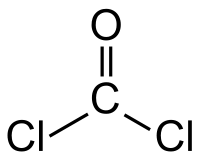
\includegraphics[width=0.15\textwidth]{_images/Phosgen.png}


	\end{enumerate}
	
	%%%%%%%%%%%%%%%%%%%%%%%%%%%%%%%%%%%%%%%%%%%%%%%%%%%%%%%%
	
	\item Ein unbekannter Stoff liefert eine Elementaranalyse von: \ce{C}: 68.13\%,
	\ce{H}: 13.72\%, \ce{O}: 18.15\% (Massenprozent). \\
	Bestimmen sie die Molek�lformel dieser Verbindung. \\
	Zeichnen sie mindestens drei reale Molek�le, die der Molek�lformel entsprechen.
	
	\begin{enumerate}

		\item 
		$M_{\ce{C}}	=12\frac{g}{Mol}$\\
		$M_{\ce{H}}	=1\frac{g}{Mol}$\\
		$M_{\ce{O}}	=16\frac{g}{Mol}$\\ 
		
		$\ce{C}:	\frac{68,13}{12}		=5,72Mol\%$\\
		$\ce{H}:	\frac{13,72}{1}		=13,72Mol\%$\\
		$\ce{O}:	\frac{18,15}{16}		=1,13Mol\%$\\ 
		
		$5,72 : 13,72 : 1,13 \Rightarrow 5:12:1 \Rightarrow \ce{C5H12O}$
		
		\item

	\begin{minipage}{0.2\textwidth}%
		\centering
		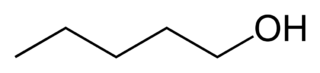
\includegraphics[width=\textwidth]{_images/Pentanol}%
	\end{minipage}%
	\hspace{1cm}
	\begin{minipage}{0.2\textwidth}%
		\centering
		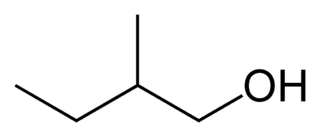
\includegraphics[width=\textwidth]{_images/2-Methyl-1-butanol}
	\end{minipage}%
	\hspace{1cm}
	\begin{minipage}{0.2\textwidth}%
		\centering
		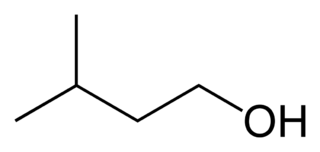
\includegraphics[width=\textwidth]{_images/3-Methyl-1-butanol}%
	\end{minipage}%
		
		
	\end{enumerate}
	
	%%%%%%%%%%%%%%%%%%%%%%%%%%%%%%%%%%%%%%%%%%%%%%%%%%%%%%%%

	\item Beschreiben Sie anhand einer Skizze s�mtliche Bindungen in Ethylen
	mit Hilfe des Konzepts der Hybridisierung. Bezeichnen Sie die Orbitale
	die Sie zeichnen.
	
	\begin{enumerate}
	
		\item 
		Eine sigma-bindung ist eine einfachbindung zwischen zwei Atomen. 
		
		hier im ethen w�ren das die bindungen zu den wasserstoffatomen 
		und eine bindung zwischen den kohlenstoffatomen. 
		
		die $\pi$-bindung ist bei doppel- und dreifachbindungen vorhanden. zus�tzlich zur einen $\sigma$-bindung. 
		
		bei der $\pi$-bindung �berlappen zwei p-orbitale, also nicht hybridisierte...  
		
		da im ethen ja nur eine doppelbindung vorhanden ist, brauchst du also nur ein nichthybridisiertes p-orbital pro 
		Kohlenstoffatom. 
		also k�nnen die zwei anderen p-orbitale mit dem s orbital hybridisieren und man erh�lt: 
		sp2 davon h�tten wir ja dann drei st�ck pro C-Atom. 
		
		und das passt ja dann auch: zwei bindungen zu wasserstoffatomen und eine bindung zum anderen kohlenstoffatom. 
		und die zwei p-orbitale �berlappen einander und bilden zweite bindung, die doppelbindung

		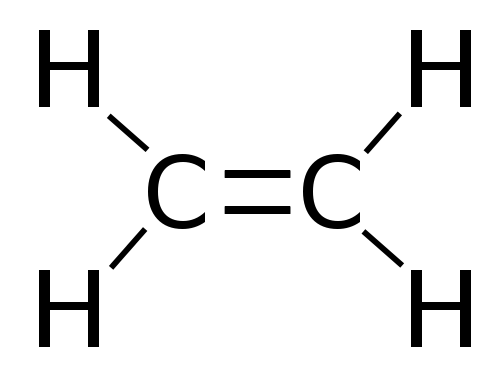
\includegraphics[width=0.2\textwidth]{_images/Ethen.png}	% angle width height scale
	
	\end{enumerate}
	
	%%%%%%%%%%%%%%%%%%%%%%%%%%%%%%%%%%%%%%%%%%%%%%%%%%%%%%%%
	
	\item Zeichnen sie das Molek�lorbitalschema f�r \ce{O2}.
	
	\begin{enumerate}
	\item 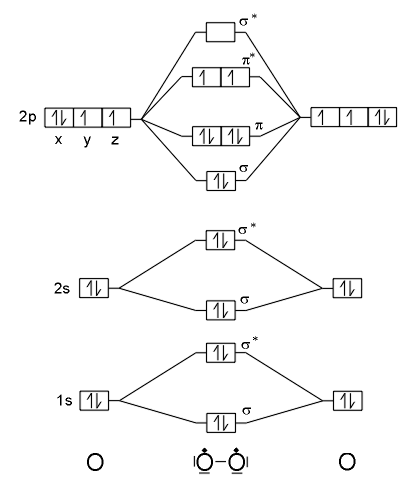
\includegraphics[width=0.5\textwidth]{_images/sauermo.png}
	
	\end{enumerate}
	
	%%%%%%%%%%%%%%%%%%%%%%%%%%%%%%%%%%%%%%%%%%%%%%%%%%%%%%%%
	
	\item Eine Verbindung, die aus 2.1\% \ce{H}, 29.8\% \ce{N} und 68,1\% \ce{O} besteht, hat
	ein Molekulargewicht von ca. 50 g/Mol. \\
	Wie lautet die Molek�lformel der Verbindung? \\
	Zeichnen sie die Lewis-Formel, wenn \ce{H} an \ce{O} gebunden ist. \\
	Wie ist die Struktur des Molek�ls? \\
	Wie ist die Hybridisierung der Orbitale am \ce{N}-Atom? \\
	Wie viele $\sigma$ - und $\pi$ -Bindungen gibt es in dem Molek�l?
	
	\begin{enumerate}
	
		\item 
		$M_{\ce{H}}	=1\frac{g}{Mol}$\\
		$M_{\ce{N}}	=14\frac{g}{Mol}$\\
		$M_{\ce{O}}	=16\frac{g}{Mol}$\\ 
		
		$\ce{H}:	\frac{2,1}{1}		=2,1Mol\%$\\
		$\ce{N}:	\frac{29,8}{14}		=2,13Mol\%$\\
		$\ce{O}:	\frac{68,1}{16}		=4,26Mol\%$\\ 
		
		$2,1 : 2,13 : 4,26 \Rightarrow 1:1:2 \Rightarrow \ce{HNO2}$
		
		\item
		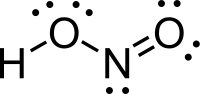
\includegraphics[width=0.2\textwidth]{_images/Lewis_Formel_Salpetrige_Saeure.png}
		
		\item
		Die Struktur ist trigonal eben.
		
		\item
		sp$^{2}$-Hybridisierung um N
		
		\item
		3 $\sigma$-Bindungen und 1 $\pi$-Bindung
		
	
	\end{enumerate}

	%%%%%%%%%%%%%%%%%%%%%%%%%%%%%%%%%%%%%%%%%%%%%%%%%%%%%%%%
	
\end{enumerate}




		%%%%%%%%%%%%%%%%%%%%%%%%%%%%%%%%%%%%%%%%%%%%%%%%%%%%%%%%%%%%%%%%%%%%%%%%%%
%%%%%%%%%%%%%%%%%%%%%%%%%%%%%%%%%%%%%%%%%%%%%%%%%%%%%%%%%%%%%%%%%%%%%%%%%%
\section*{GASE \& FL�SSIGKEITEN \& L�SUNGEN}
%%%%%%%%%%%%%%%%%%%%%%%%%%%%%%%%%%%%%%%%%%%%%%%%%%%%%%%%%%%%%%%%%%%%%%%%%%
%%%%%%%%%%%%%%%%%%%%%%%%%%%%%%%%%%%%%%%%%%%%%%%%%%%%%%%%%%%%%%%%%%%%%%%%%%

%%%%%%%%%%%%%%%%%%%%%%%%%%%%%%%%%%%%%
	\begin{karte}{
		Eine Gasmischung aus 6.00 g \ce{O2} und 9.00 g \ce{CH4} wird bei 0�C in einen Beh�lter (V = 100 mL) gegeben. \\
		Wie sind die Partialdr�cke f�r jedes Gas und wie ist der Gesamtdruck im Beh�lter in atm? \\
		$R = 0.0821  \frac{L\,atm}{Mol \,K}$
		}
		
		\begin{enumerate}
			
				\item 
				$M_{\ce{O2}}		=2\cdot16								=32\frac{g}{Mol}$\\
				$M_{\ce{CH4}}	=12+4\cdot1							=16\frac{g}{Mol}$\\
				$n_{\ce{O2}}		=\frac{6g}{32\frac{g}{Mol}}		=0,1875 Mol$\\
				$n_{\ce{CH4}}	=\frac{9g}{16\frac{g}{Mol}}		=0,5625 Mol$
				
				$\displaystyle pV=nRT \Rightarrow p=\frac{nRT}{V}$\\
						
				$\displaystyle P_{\ce{O2}}		=\frac{0,1875Mol\cdot0,0821\frac{L\,atm}{Mol \,K}\cdot273,15K}{0,1L}	=42atm$\\
				$\displaystyle P_{\ce{CH4}}	=\frac{0,5625Mol\cdot0,0821\frac{L\,atm}{Mol \,K}\cdot273,15K}{0,1L}	=126atm$
		
				$\displaystyle p_{ges} = \sum_{i=1}^k p_i$
				
				$P_{ges}					=42atm + 126atm					=168atm$
				
			\end{enumerate}
		
	\end{karte}
%%%%%%%%%%%%%%%%%%%%%%%%%%%%%%%%%%%%%

%%%%%%%%%%%%%%%%%%%%%%%%%%%%%%%%%%%%%
	\begin{karte}{
		Ammoniumnitrit zersetzt sich beim Erhitzen zu \ce{N2} Gas: \ce{NH4NO2 -> N_{2(g)} + 2H2O_{(l)}} 
		Wenn eine Probe in einem Reagenzglas zersetzt wird, werden 511 mL \ce{N2}-Gas �ber Wasser bei 26�C und 745 Torr Gesamtdruck aufgefangen. \\
		
		Wie viel Gramm Ammoniumnitrit wurden zersetzt? \\
		$R = 62,36 \frac{L\,torr}{Mol \,K}$
		}
		
		\begin{enumerate}
		
				\item 
				$M_{\ce{NH4NO2}}		=14+4\cdot1+14+2\cdot16	=64\frac{g}{Mol}$ 
				
				$\displaystyle n			=\frac{P\cdot V}{R\cdot T}		
									=\frac{745Torr \cdot 0,511 L}{62,36  \frac{L\,torr}{Mol \,K} \cdot (273,15+26)K}
									=0,02Mol$
				
				$m_{\ce{NH4NO2}}		=64\frac{g}{Mol} \cdot 0,02Mol		=1,28g$
				
			\end{enumerate}
		
	\end{karte}
%%%%%%%%%%%%%%%%%%%%%%%%%%%%%%%%%%%%%

%%%%%%%%%%%%%%%%%%%%%%%%%%%%%%%%%%%%%
	\begin{karte}{
		Cyclopropan, besteht aus 85.7 Massen\% \ce{C} und 14.3 Massen\% \ce{H}. 
			Wenn 1.56 g Cyclopropan ein Volumen von 1 L bei 0.984 atm und 50�C hat, 
			wie ist dann die Molek�lformel von Cyclopropan? \\
			W�rden Sie erwarten, dass Cyclopropan mehr oder weniger als Argon vom idealen Gasverhalten bei moderaten Dr�cken und Zimmertemperatur abweicht? \\
			Erkl�ren Sie! \\
			$R = 0.0821  \frac{L\,atm}{Mol \,K}$
		}
		
		\begin{enumerate}
			
				\item
				$M_{\ce{C}}	=12 \frac{g}{Mol}$ \\
				$M_{\ce{H}}	=1 \frac{g}{Mol}$ \\
			
			\end{enumerate}
		
	\end{karte}
%%%%%%%%%%%%%%%%%%%%%%%%%%%%%%%%%%%%%

%%%%%%%%%%%%%%%%%%%%%%%%%%%%%%%%%%%%%
	\begin{karte}{
		9.23 g einer Mischung von Magnesiumcarbonat und Calciumoxid wird mit einem �berschuss von Salzs�ure behandelt. Die resultierende Reaktion erzeugt 1.72 L Kohlendioxid bei 28�C und 743 Torr. \\
		Schreiben Sie ausgeglichene chemische Gleichungen f�r die Reaktionen, die zwischen der Salzs�ure und jedem Bestandteil der Mischung auftreten. \\
		Berechnen sie die Gesamtmolzahl von Kohlendioxid, die durch diese Reaktion gebildet wird. \\
		Unter der Annahme, dass die Reaktionen vollst�ndig ablaufen, berechnen sie die Massenprozent von Magnesiumcarbonat in der Mischung.\\
		(R = 62.36 L torr/Mol K)
		}
		
	\end{karte}
%%%%%%%%%%%%%%%%%%%%%%%%%%%%%%%%%%%%%

%%%%%%%%%%%%%%%%%%%%%%%%%%%%%%%%%%%%%
	\begin{karte}{
		Zeichnen und beschreiben Sie das Phasendiagramm von Wasser. \\
		Definieren Sie die beiden besonderen Punkte.
		}
		
	\end{karte}
%%%%%%%%%%%%%%%%%%%%%%%%%%%%%%%%%%%%%

%%%%%%%%%%%%%%%%%%%%%%%%%%%%%%%%%%%%%
	\begin{karte}{
		Welche Art von Anziehungskr�ften liegt zwischen Teilchen in \\
			a) molekularen Kristallen, \\
			b) kovalenten Kristallen, \\
			c) ionischen Kristallen und\\
			d) metallischen Kristallen vor?
		}
		
	\end{karte}
%%%%%%%%%%%%%%%%%%%%%%%%%%%%%%%%%%%%%

%%%%%%%%%%%%%%%%%%%%%%%%%%%%%%%%%%%%%
	\begin{karte}{
		Wie unterscheidet ein amorpher Festk�rper sich von einem kristallinen?\\
		Geben Sie je ein Beispiel f�r einen amorphen und einen kristallinen Festk�rper.
		}
		
	\end{karte}
%%%%%%%%%%%%%%%%%%%%%%%%%%%%%%%%%%%%%

%%%%%%%%%%%%%%%%%%%%%%%%%%%%%%%%%%%%%
	\begin{karte}{
		Glycerin ist ein wasserl�slicher Nichtelektrolyt mit einer Dichte
			von 1.26 g/mL bei 25�C. Berechnen sie den Dampfdruck einer
			L�sung, die durch Zugabe von 50 mL Glycerin zu 500 mL Wasser hergestellt
			wird. Der Dampfdruck von reinem Wasser bei 25�C betr�gt
			23.8 Torr.
		}
		
	\end{karte}
%%%%%%%%%%%%%%%%%%%%%%%%%%%%%%%%%%%%%

%%%%%%%%%%%%%%%%%%%%%%%%%%%%%%%%%%%%%
	\begin{karte}{
		Der Dampfdruck von reinem Wasser bei 110�C ist 1070 Torr.
			Eine L�sung aus Ethylenglykol und Wasser hat einen Dampfdruck von
			1.00 atm bei 110�C. Berechnen Sie den Molenbruch von Ethylenglykol.
		}
		
	\end{karte}
%%%%%%%%%%%%%%%%%%%%%%%%%%%%%%%%%%%%%

%%%%%%%%%%%%%%%%%%%%%%%%%%%%%%%%%%%%%
	\begin{karte}{
		Wenn 10.0 g \ce{Hg(NO3)2} in 1 kg Wasser aufgel�st wird, ist der
			Gefrierpunkt der L�sung -0.162 �C. Wenn 10.0 g \ce{HgCl2}
			in 1 kg Wasser gel�st werden, gefriert die L�sung bei -0.0685�C.
			Bestimmen sie anhand der dieser Daten, welches der st�rkere Elektrolyt
			ist und berechnen sie die Siedepunktserh�hung in beiden F�llen. ($K_{b\,\ce{H2O}}$
			= 0.51 �C/m)
		}
		
	\end{karte}
%%%%%%%%%%%%%%%%%%%%%%%%%%%%%%%%%%%%%



		%!TEX root = ../chemie.tex



\newpage

\chapter{CHEMISCHE KINETIK}
\begin{enumerate}

	%%%%%%%%%%%%%%%%%%%%%%%%%%%%%%%%%%%%%%%%%%%%%%%%%%%%%%%%
	
	\item F�r die Reaktion \ce{BF_{3(g)} + NH_{3(g)} -> F_{3}BNH_{3(g)}}
	wurden folgende Daten gemessen:\\
	 %
	\begin{tabular}{cccc}
	\hline 
	Versuch & \ce{BF_{3}} / $\frac{M}{L}$ & \ce{NH3} / $\frac{M}{L}$ & Anfangsreaktionsgeschw $\frac{M}{s}$ \tabularnewline
	\hline 
	\hline 
	1 & 0,25 & 0,25 & 0,1230\tabularnewline
	\hline 
	2 & 0,250 & 0,125 & 0,1065\tabularnewline
	\hline 
	3 & 0,200 & 0,100 & 0,0682\tabularnewline
	\hline 
	4 & 0,350 & 0,100 & 0,1193\tabularnewline
	\hline 
	5 & 0,175 & 0,100 & 0,0596\tabularnewline
	\hline 
	\end{tabular}\\
	Wie lautet das Geschwindigkeitsgestz f�r die Reaktion? Was ist die
	Gesamtordnung der Reaktion? Was ist der Wert f�r die Geschwindigkeitskonstante
	der Reaktion?
	
	\begin{enumerate}
	\item a
	\end{enumerate}
	\item Die Aktivierungsenergie einer bestimmten Reaktion ist $65.7kJ/Mol$.
	Wie viel schneller findet die Reaktion bei Die Zersetzung von Wasserstoffperoxid
	wird durch Jodidionen katalysiert. Man glaubt, dass die katalysierte
	Reaktion �ber einen zweistufigen Mechanismus abl�uft:
	\ce{H2O2 + I- -> H2O + IO-} (langsam) und \ce{IO- + H2O2 -> H2O + O2 + I-}
	(schnell) Schreiben Sie das Geschwindigkeitsgesetz f�r jede der
	Elementarreaktionen des Reaktionsmechanismuses an. 
	Schreiben Sie die chemische Gleichung f�r den Gesamtprozess. 
	Sagen Sie das Geschwindigkeitsgesetz f�r den Gesamtprozess vorher.
	
	\begin{enumerate}
	\item a
	\end{enumerate}
	\item Der erste Schritt eines Mechanismus bei der Reaktion von Brom ist:
	\ce{Br2 <-> 2Br} (schnell, im Gleichgewicht)\\
	Wie lautet der Ausdruck, der die Konzentration von \ce{Br} mit der von
	\ce{Br2} in Beziehung setzt?
	
	\begin{enumerate}
	\item a
	\end{enumerate}
	\item Viele metallische Katalysatoren, vor allem Edelmetallkatalysatoren,
	werden h�ufig als sehr d�nne Schichten auf einer Substanz mit hoher
	spezifischer Oberfl�che, wie Aluminiumoxid oder Siliziumoxid abgeschieden.
	Warum ist das ein effektives Verfahren zur Nutzung von Katalysatorstoffen?
	
	\begin{enumerate}
	\item a
	\end{enumerate}
	\end{enumerate}
	
	

%%%%%%%%%%%%%%%%%%%%%%%%%%%%%%%%%%%%%%%%%%%%%%%%%%%%%%%%





		%%%%%%%%%%%%%%%%%%%%%%%%%%%%%%%%%%%%%%%%%%%%%%%%%%%%%%%%%%%%%%%%%%%%%%%%%%
%%%%%%%%%%%%%%%%%%%%%%%%%%%%%%%%%%%%%%%%%%%%%%%%%%%%%%%%%%%%%%%%%%%%%%%%%%
\section*{CHEMISCHES GLEICHGEWICHT}
%%%%%%%%%%%%%%%%%%%%%%%%%%%%%%%%%%%%%%%%%%%%%%%%%%%%%%%%%%%%%%%%%%%%%%%%%%
%%%%%%%%%%%%%%%%%%%%%%%%%%%%%%%%%%%%%%%%%%%%%%%%%%%%%%%%%%%%%%%%%%%%%%%%%%

%%%%%%%%%%%%%%%%%%%%%%%%%%%%%%%%%%%%%
	\begin{karte}{
		
		Bestimmen Sie mit folgenden Informationen:\\
		\ce{HF <-> H+ + F-} $K_{c}=6.8 \cdot 10^{-4}$ und\\
		\ce{H2C2O4 <-> 2H+ + C2O4^{2-}} $K_{c}=3,8 \cdot 10^{-6}$\\
		die Gleichgewichtskonstante $K_{c}$ der Reaktion  \ce{2HF + C2O4^{2-} <-> 2F- + H2C2O4} (alle Reaktionspartner sind aquatisiert). Zeichnen sie eine plausible Lewis-Strukturformel von \ce{H2C2O4}.
		
		}
		
	\end{karte}
%%%%%%%%%%%%%%%%%%%%%%%%%%%%%%%%%%%%%

%%%%%%%%%%%%%%%%%%%%%%%%%%%%%%%%%%%%%
	\begin{karte}{
		
		Die Gleichgewichtskonstanten $K_{p}$ (bei 700�C) f�r die Reaktionen:\\
		\ce{H2 +I2 <-> 2HI} $K_{p}=54.0$,\\
		\ce{N2 + 3H2 <-> 2NH3} $K_{p}=1,04\cdot10^{-4}$ \\
		sind gegeben. Bestimmen Sie den Wert f�r $K_{p}$ f�r die Reaktion \ce{2NH3 + 3I2 <-> 6HI + N2} bei $700K$. (Alle Reaktionspartner sind im gasf�rmigen Zustand).
		
		}
		
	\end{karte}
%%%%%%%%%%%%%%%%%%%%%%%%%%%%%%%%%%%%%

%%%%%%%%%%%%%%%%%%%%%%%%%%%%%%%%%%%%%
	\begin{karte}{
		
		Schwefeltrioxid zersetzt sich bei hoher Temperatur in einem geschlossenen Beh�lter gem��: \ce{2SO3 <-> 2SO2 + O2} (Alle Reaktionspartner sind im gasf�rmigen Zustand). Ein Gef�� wird bei $1000K$ mit \ce{SO_{3}} bei einem Partialdruck von $0,500atm$ gef�llt. Im Gleichgewicht ist der Partialdruck von \ce{SO3} $0,200atm$. Berechnen sie den Wert f�r $K_{p}$ bei $1000K$.
		
		}
		
	\end{karte}
%%%%%%%%%%%%%%%%%%%%%%%%%%%%%%%%%%%%%

%%%%%%%%%%%%%%%%%%%%%%%%%%%%%%%%%%%%%
	\begin{karte}{
		
		Bei 1000 K ist der Wert f�r $K_{p}$ der Reaktion \\
		\ce{2SO3 <->2SO2 + O2}\\
		gleich $0,338$. Sagen sie vorher welche Reaktion abl�uft, wenn ein Gemisch mit den Anfangspartialdr�cken von \\
		$p_{\ce{SO3}}=0,16atm$; \\
		$p_{\ce{SO2}}=0.41atm$; \\
		$p_{\ce{O2}}=2.5atm$ betrachtet wird.
		
		}
		
	\end{karte}
%%%%%%%%%%%%%%%%%%%%%%%%%%%%%%%%%%%%%

%%%%%%%%%%%%%%%%%%%%%%%%%%%%%%%%%%%%%
	\begin{karte}{
		
		Schreiben sie den Gleichgewichtsausdruck f�r das Gleichgewicht: \ce{C_{(s)} + CO2_{(g)} <-> 2CO_{(g)}}.
		Die unten angef�hrte Tabelle zeigt die Molprozente von \ce{CO2} und \ce{CO} bei einem Gesamtdruck von 1 atm f�r mehrere Temperaturen.
		Berechnen sie den Wert von Kp bei jeder Temperatur. 
		Ist die Reaktion exotherm oder endotherm? 
		Begr�nden sie Ihre Antwort. (R = 0.0821 L atm/Mol K).

		\begin{tabular}{ccc}
			\hline 
			$Temperatur$ & $CO_{2}$ & $CO$ \tabularnewline
			$\celsius $ & $Mol\%$ & $Mol\%$ \tabularnewline
			\hline 
			\hline 
			$850$ & $6,23$ & $93,77$ \tabularnewline
			$950$ & $1,32$ & $98,68$ \tabularnewline
			$1050$ & $0,37$ & $99,63$ \tabularnewline
			\hline 
		\end{tabular}
		
		}
		
	\end{karte}
%%%%%%%%%%%%%%%%%%%%%%%%%%%%%%%%%%%%%

%%%%%%%%%%%%%%%%%%%%%%%%%%%%%%%%%%%%%
	\begin{karte}{
		
		F�r das Gleichgewicht \ce{PCl5 <-> PCl3 + Cl2} (Alle Reaktionspartner sind im gasf�rmigen Zustand) betr�gt Kp @ 500K 0.497. \\
		Eine Gasflasche wird bei einem Anfangsdruck von 1.66 atm gef�llt.\\
		Was sind die Gleichgewichtsdr�cke f�r die drei Gase bei dieser Temperatur?
		
		}
		
	\end{karte}
%%%%%%%%%%%%%%%%%%%%%%%%%%%%%%%%%%%%%


		%%%%%%%%%%%%%%%%%%%%%%%%%%%%%%%%%%%%%%%%%%%%%%%%%%%%%%%%%%%%%%%%%%%%%%%%%%
%%%%%%%%%%%%%%%%%%%%%%%%%%%%%%%%%%%%%%%%%%%%%%%%%%%%%%%%%%%%%%%%%%%%%%%%%%
\section*{S�URE-BASE GLEICHGEWICHTE}
%%%%%%%%%%%%%%%%%%%%%%%%%%%%%%%%%%%%%%%%%%%%%%%%%%%%%%%%%%%%%%%%%%%%%%%%%%
%%%%%%%%%%%%%%%%%%%%%%%%%%%%%%%%%%%%%%%%%%%%%%%%%%%%%%%%%%%%%%%%%%%%%%%%%%


%%%%%%%%%%%%%%%%%%%%%%%%%%%%%%%%%%%%%
	\begin{karte}{
		
		Der pH-Wert von 0.62 g Niacin in 250 mL Wasser betr�gt bei 25�C 3.26. Wie gro� ist die S�urekonstante $K_{s}$ und wie viel Prozent Nicatin sind unter diesen Bedingungen dissoziiert?\\
		
\includegraphics{_images/1.pdf}
		
		}
		
	\end{karte}
%%%%%%%%%%%%%%%%%%%%%%%%%%%%%%%%%%%%%

%%%%%%%%%%%%%%%%%%%%%%%%%%%%%%%%%%%%%
	\begin{karte}{
		
	Berechnen sie den Prozentsatz an dissoziierten \ce{HF} Molek�len in w�ssrigen \ce{HF}-L�sungen von 0.10 Mol/L und von 0.01 Mol/L. $K_{S}=6,8\cdot10^{-4}$
		
		}
		
	\end{karte}
%%%%%%%%%%%%%%%%%%%%%%%%%%%%%%%%%%%%%

%%%%%%%%%%%%%%%%%%%%%%%%%%%%%%%%%%%%%
	\begin{karte}{
		
		Berechnen sie den pH-Wert einer Oxals�urel�sung \ce{(COOH)_{2}} mit einer Konzentration von 0.020 Mol/L bei 25�C. $K{}_{S1}=5,9\cdot10^{-2}$;
		$K_{S2}=6,4\cdot10^{-5}$. Bestimmen Sie die Konzentration des Oxalations \ce{(COO)_{2}^{2-}} in der L�sung.
		
		}
		
	\end{karte}
%%%%%%%%%%%%%%%%%%%%%%%%%%%%%%%%%%%%%

%%%%%%%%%%%%%%%%%%%%%%%%%%%%%%%%%%%%%
	\begin{karte}{
		
		Phosphorige S�ure \ce{(H_{3}PO_{3})} besitzt die rechts gezeigte Lewis Strukturformel: Erkl�ren Sie, warum \ce{H3PO3} zweibasig und nicht dreibasig ist. Es werden 25 mL \ce{H_{3}PO_{3}} mit einer 0.102 Mol/L \ce{NaOH}-L�sung titriert. Dabei werden 23.3 mL dieser L�sung ben�tigt um die \ce{H3PO3} zu neutralisieren. Welche Molarit�t hat die \ce{H3PO3}-L�sung? Der pH-Wert der L�sung betr�gt 1.59. 
		
		Berechnen sie $K_{S1}$ und den Dissoziationsgrad unter der Annahme, dass $K_{S2}$ vernachl�ssigt werden kann.\\
		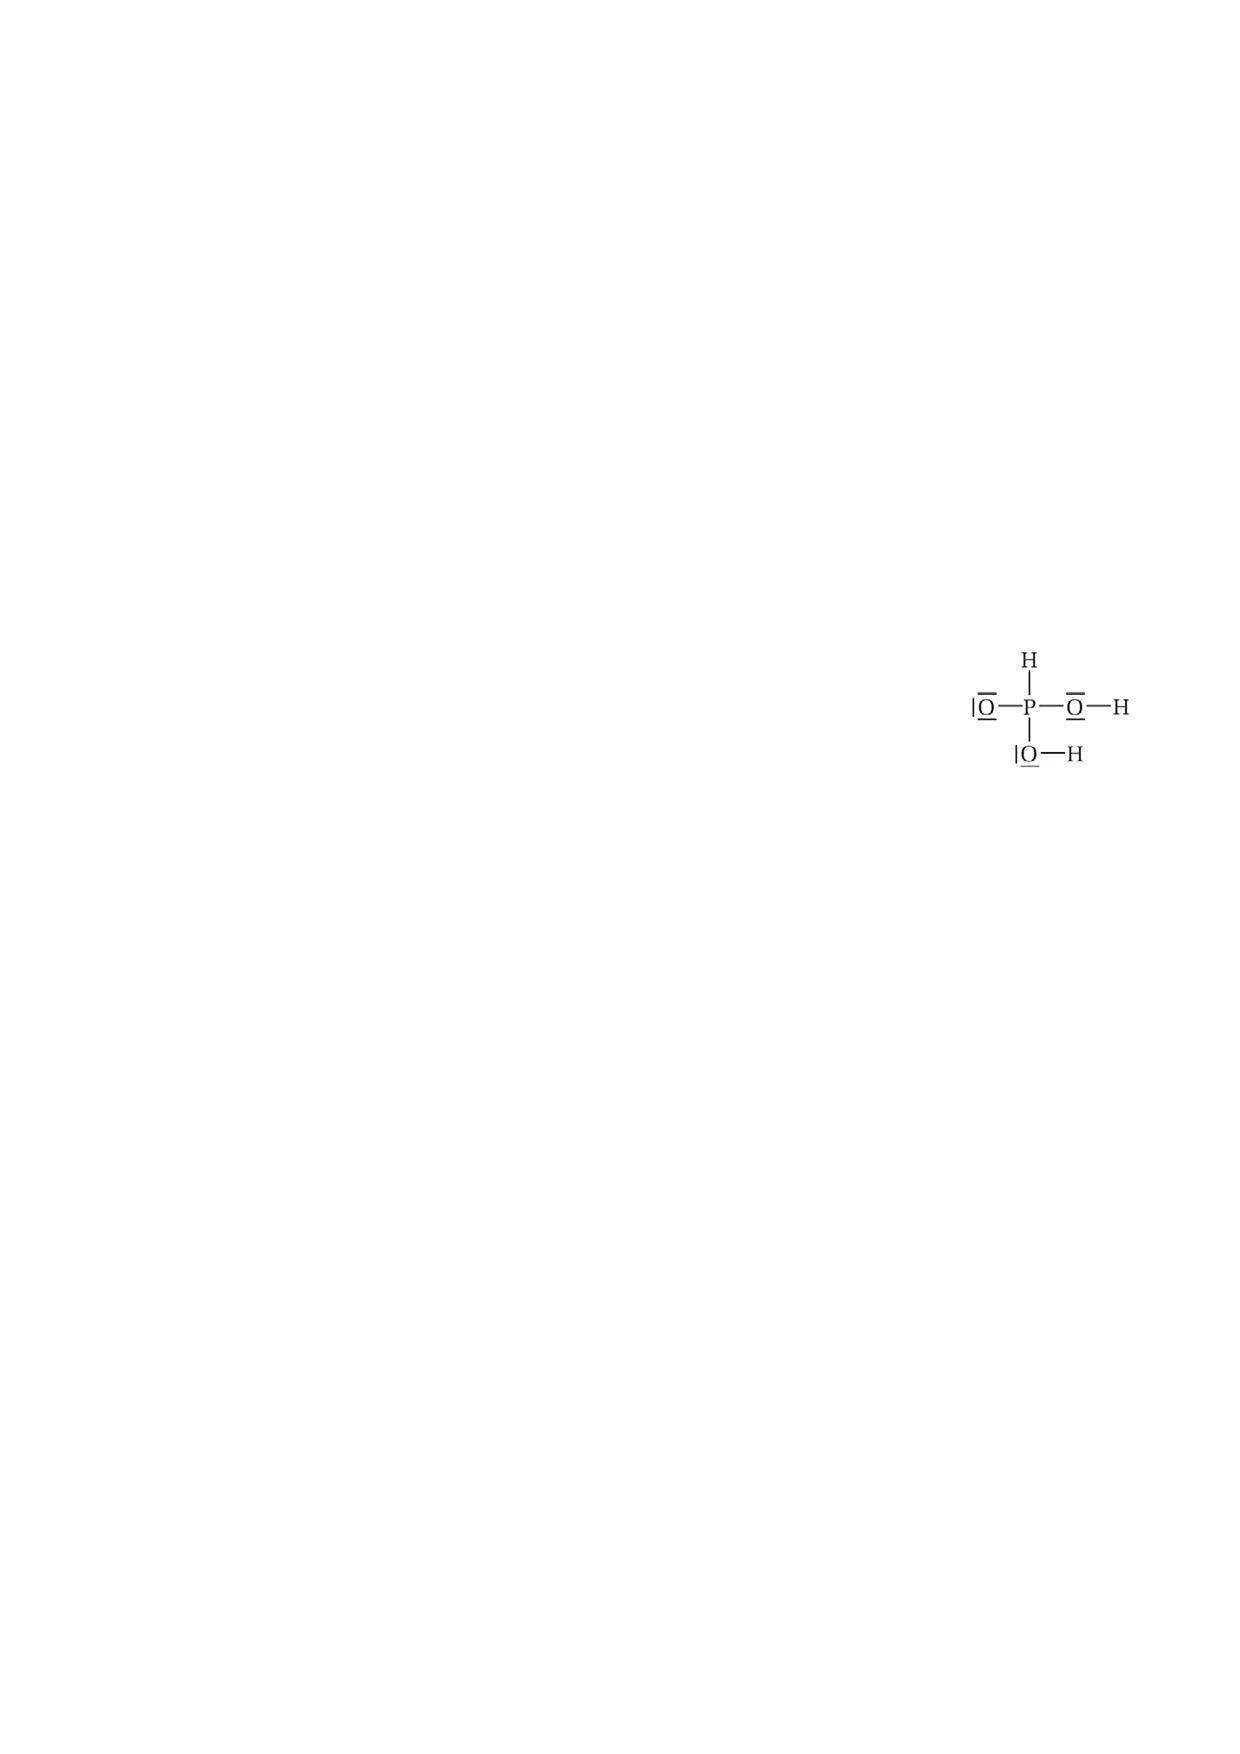
\includegraphics[width=0.3\textwidth, angle=0]{_images/2.pdf}
		
		
		}
		
	\end{karte}
%%%%%%%%%%%%%%%%%%%%%%%%%%%%%%%%%%%%%

%%%%%%%%%%%%%%%%%%%%%%%%%%%%%%%%%%%%%
	\begin{karte}{
		
		Berechnen Sie die Konzentration des Fluoridions und den pH-Wert einer L�sung mit 0.20 Mol/L \ce{HF} und 0.10 Mol/L \ce{HCl}. $(K_{S\, HF}=6,8\cdot10^{-4})$
		
		}
		
	\end{karte}
%%%%%%%%%%%%%%%%%%%%%%%%%%%%%%%%%%%%%

%%%%%%%%%%%%%%%%%%%%%%%%%%%%%%%%%%%%%
	\begin{karte}{
		
		Welchen pH-Wert hat eine L�sung aus 0.30 Mol Essigs�ure und 0.30 Mol Natriumacetat, zu denen soviel Wasser gegeben wird, dass 1.0 L L�sung entsteht? $(K_{S\, Essigs\ddot{a}ure}=1,8\cdot10^{-5})$
		
		}
		
	\end{karte}
%%%%%%%%%%%%%%%%%%%%%%%%%%%%%%%%%%%%%

%%%%%%%%%%%%%%%%%%%%%%%%%%%%%%%%%%%%%
	\begin{karte}{
		
		Welchen pH-Wert hat ein Puffer mit 0.12 Mol/L Benzoes�ure und 0.20 Mol/L Natriumbenzoat? $(K_{S\, Benzoes\ddot{a}ure}=6,3\cdot10^{-5})$
		
		}
		
	\end{karte}
%%%%%%%%%%%%%%%%%%%%%%%%%%%%%%%%%%%%%

%%%%%%%%%%%%%%%%%%%%%%%%%%%%%%%%%%%%%
	\begin{karte}{
		
		Berechnen sie den pH-Wert. Der sich einstellt, wenn 45 mL einer 0.100 Mol/L \ce{NaOH}-L�sung zu einer 25 mL einer 0.100 Mol/L Essigs�urel�sung gegeben werden. $(K_{S\, Essigs\ddot{a}ure}=1,8\cdot10^{-5})$
		
		}
		
	\end{karte}
%%%%%%%%%%%%%%%%%%%%%%%%%%%%%%%%%%%%%

%%%%%%%%%%%%%%%%%%%%%%%%%%%%%%%%%%%%%
	\begin{karte}{
		
		Der Wert von $K_{L}$ von \ce{CaF_{2}} ist bei 25�C gleich $3.9\cdot10^{-11}Mol^{3}/L^{3}$. Berechnen Sie die L�slichkeit von \ce{CaF2} in Gramm/Liter.
		
		}
		
	\end{karte}
%%%%%%%%%%%%%%%%%%%%%%%%%%%%%%%%%%%%%

%%%%%%%%%%%%%%%%%%%%%%%%%%%%%%%%%%%%%
	\begin{karte}{
		
		Bildet sich beim Mischen von $0.1L$ $8,0\cdot10^{-3}Mol/L$ \ce{Pb(NO3)2} und $0.4L$ $5,0\cdot10^{-3}$ $Mol/L$ \ce{Na2SO4} ein Niederschlag?
		$(K_{L_{8\ce{PbSO4}}}=6,3\cdot10^{-7}Mol^{2}/L^{2})$ 
		
		}
		
	\end{karte}
%%%%%%%%%%%%%%%%%%%%%%%%%%%%%%%%%%%%%


		%%%%%%%%%%%%%%%%%%%%%%%%%%%%%%%%%%%%%%%%%%%%%%%%%%%%%%%%%%%%%%%%%%%%%%%%%%
%%%%%%%%%%%%%%%%%%%%%%%%%%%%%%%%%%%%%%%%%%%%%%%%%%%%%%%%%%%%%%%%%%%%%%%%%%
\section*{THERMODYNAMIK II}
%%%%%%%%%%%%%%%%%%%%%%%%%%%%%%%%%%%%%%%%%%%%%%%%%%%%%%%%%%%%%%%%%%%%%%%%%%
%%%%%%%%%%%%%%%%%%%%%%%%%%%%%%%%%%%%%%%%%%%%%%%%%%%%%%%%%%%%%%%%%%%%%%%%%%

%%%%%%%%%%%%%%%%%%%%%%%%%%%%%%%%%%%%%
	\begin{karte}{
		
		Sagen sie voraus, ob $\Delta$S f�r folgende Prozesse positiv oder negativ ist, wobei wir davon ausgehen, dass alle bei konstanter Temperatur ablaufen:\\
		(a) \ce{H2O_{(g)} -> H2O_{(l)}}\\
		(b) \ce{Ag_{(aq)}^{+} + Cl_{(aq)}^{-} -> AgCl_{(s)}}\\
		(c) \ce{4Fe_{(s)} + 3O2_{(g)} -> 2Fe2O3_{(s)}}\\
		(d) \ce{N2_{(g)} + O2_{(g)} -> 2NO_{(g)}}
		
		}
		
	\end{karte}
%%%%%%%%%%%%%%%%%%%%%%%%%%%%%%%%%%%%%

%%%%%%%%%%%%%%%%%%%%%%%%%%%%%%%%%%%%%
	\begin{karte}{
		
		(a) Was ist das Besondere an einem reversiblen Prozess? \\
		(b) Gehen Sie davon aus, dass ein reversibler Prozess umgekehrt wird, und das System in seinen Ausgangszustand zur�ckversetzt wird. Was l�sst sich �ber die Umgebung nach der Umkehrung des Prozesses aussagen? \\
		(c) Unter welchen Umst�nden handelt es sich beim Verdampfen von Wasser zu Dampf um einen reversiblen Prozess?
		
		}
		
	\end{karte}
%%%%%%%%%%%%%%%%%%%%%%%%%%%%%%%%%%%%%

%%%%%%%%%%%%%%%%%%%%%%%%%%%%%%%%%%%%%
	\begin{karte}{
		
		Vervollst�ndigen Sie folgende Redoxgleichung: \\
		\ce{MnO- + Fe2+ + H+ -> MnO2 + Fe^{3+} + H2O}
		
		}
		
	\end{karte}
%%%%%%%%%%%%%%%%%%%%%%%%%%%%%%%%%%%%%

%%%%%%%%%%%%%%%%%%%%%%%%%%%%%%%%%%%%%
	\begin{karte}{
	
		Vervollst�ndigen Sie folgende Redoxgleichung:\\
		\ce{MnO4- + Mn^{2+} + H+ -> MnO2 + H2O}
		
		}
		
	\end{karte}
%%%%%%%%%%%%%%%%%%%%%%%%%%%%%%%%%%%%%

%%%%%%%%%%%%%%%%%%%%%%%%%%%%%%%%%%%%%
	\begin{karte}{
		
		Vervollst�ndigen Sie folgende Redoxgleichung: \\
		\ce{Cr2O7^{2-} + CH3OH + H+ -> Cr^{3+} + CO2 + H2O}
		
		}
		
	\end{karte}
%%%%%%%%%%%%%%%%%%%%%%%%%%%%%%%%%%%%%

%%%%%%%%%%%%%%%%%%%%%%%%%%%%%%%%%%%%%
	\begin{karte}{
		
		Beschreiben sie mit Hilfe einer Skizze den Aufbau einer Alkalibatterie und Formulieren Sie die Anoden und Kathodenreaktion.
		
		}
		
	\end{karte}
%%%%%%%%%%%%%%%%%%%%%%%%%%%%%%%%%%%%%

%%%%%%%%%%%%%%%%%%%%%%%%%%%%%%%%%%%%%
	\begin{karte}{
		
		Beschreiben sie mit Hilfe einer Skizze die Korrosion von Eisen und formulieren Sie die Anoden und Kathodenreaktion, sowie die Gesamtreaktion.
		
		}
		
	\end{karte}
%%%%%%%%%%%%%%%%%%%%%%%%%%%%%%%%%%%%%



		%!TEX root = ../chemie.tex




\newpage

\chapter{STOFFCHEMIE}

\begin{enumerate}

	%%%%%%%%%%%%%%%%%%%%%%%%%%%%%%%%%%%%%%%%%%%%%%%%%%%%%%%%
	
	\item Beschreiben sie Eigenschaften und Verwendung von Schwefel und Selen.
	
	\begin{enumerate}
		\item a
	\end{enumerate}

	%%%%%%%%%%%%%%%%%%%%%%%%%%%%%%%%%%%%%%%%%%%%%%%%%%%%%%%%
	\item Beschreiben sie die Herstellung und Verwendung von Stickstoff.
	
	\begin{enumerate}
		\item a
	\end{enumerate}

	%%%%%%%%%%%%%%%%%%%%%%%%%%%%%%%%%%%%%%%%%%%%%%%%%%%%%%%%

	\item Beschreiben sie Vorkommen und Herstellung von Silizium.
	
	\begin{enumerate}
		\item a
	\end{enumerate}

	%%%%%%%%%%%%%%%%%%%%%%%%%%%%%%%%%%%%%%%%%%%%%%%%%%%%%%%%

	\item Beschreiben sie die Herstellung von Stahl. Zeichnen sie drei Isomere
	der Summenformel \ce{C5H12} und geben sie einen chemischen Namen f�r jede
	
	\begin{enumerate}
		\item a
	\end{enumerate}

	%%%%%%%%%%%%%%%%%%%%%%%%%%%%%%%%%%%%%%%%%%%%%%%%%%%%%%%%

	\item Zeichnen sie die Strukturformeln des cis- und des trans-Isomers von
	3- Penten-1-ol. Kann bei Cyclopenten eine cis-trans Isomerie vorliegen?
	Erkl�ren sie ihre Antwort.
	
	\begin{enumerate}
		\item a
	\end{enumerate}

	%%%%%%%%%%%%%%%%%%%%%%%%%%%%%%%%%%%%%%%%%%%%%%%%%%%%%%%%

	\item Beschreiben Sie die sechs Kohlenwasserstofffraktionen der Erd�ldestillation,
	deren Siedepunktsbereiche und deren Verwendung.
	
	\begin{enumerate}
		\item a
	\end{enumerate}

	%%%%%%%%%%%%%%%%%%%%%%%%%%%%%%%%%%%%%%%%%%%%%%%%%%%%%%%%

	\item Beschreiben Sie die molekulare Grundlage unserer Sehf�higkeit.
	
	\begin{enumerate}
		\item a
	\end{enumerate}

	%%%%%%%%%%%%%%%%%%%%%%%%%%%%%%%%%%%%%%%%%%%%%%%%%%%%%%%%

	\item Definieren Sie Chiralit�t und zeichnen Sie ein beliebiges chirales
	Molek�l.
	
	\begin{enumerate}
		\item a
	\end{enumerate}

	%%%%%%%%%%%%%%%%%%%%%%%%%%%%%%%%%%%%%%%%%%%%%%%%%%%%%%%%

	\item Zeichnen Sie drei beliebige nat�rliche Aminos�uren und beschreiben
	Sie die Natur der Peptidbindung.
	
	\begin{enumerate}
		\item a
	\end{enumerate}

	%%%%%%%%%%%%%%%%%%%%%%%%%%%%%%%%%%%%%%%%%%%%%%%%%%%%%%%%

	\item Zeichnen Sie die Wiederholeinheit von Polyethylen, Polystyrol und
	Nylon 6,6. Geben sie je zwei Anwendungsgebiete dieser Kunststoffe
	an.

	\begin{enumerate}
		\item a
	\end{enumerate}
		
	%%%%%%%%%%%%%%%%%%%%%%%%%%%%%%%%%%%%%%%%%%%%%%%%%%%%%%%%

\end{enumerate}



%%%%%%%%%%%%%%%%%%%%%%%%%%%%%%%%%%%%%%%%%%%%%%%%%%%%%%%%



		%%%%%%%%%%%%%%%%%%%%%%%%%%%%%%%%%%%%%%%%%%%%%%%%%%%%%%%%%%%%%%%%%%%%%%%%%%
%%%%%%%%%%%%%%%%%%%%%%%%%%%%%%%%%%%%%%%%%%%%%%%%%%%%%%%%%%%%%%%%%%%%%%%%%%
\section*{ALLGEMEINE FRAGEN}
%%%%%%%%%%%%%%%%%%%%%%%%%%%%%%%%%%%%%%%%%%%%%%%%%%%%%%%%%%%%%%%%%%%%%%%%%%
%%%%%%%%%%%%%%%%%%%%%%%%%%%%%%%%%%%%%%%%%%%%%%%%%%%%%%%%%%%%%%%%%%%%%%%%%%

%%%%%%%%%%%%%%%%%%%%%%%%%%%%%%%%%%%%%
\begin{karte}{
	%Frage
	Wie ist das Periodensystem aufgebaut und welche Informationen kann man daraus ablesen.

	}
	%Antwort
	Antwort

\end{karte}
%%%%%%%%%%%%%%%%%%%%%%%%%%%%%%%%%%%%%

%%%%%%%%%%%%%%%%%%%%%%%%%%%%%%%%%%%%%
\begin{karte}{
	
	Welche chemischen Bindungen kennen Sie? Geben Sie zu jeder ein Beispiel und erkl�ren Sie.
	
	}
	
	Antwort
	
\end{karte}
%%%%%%%%%%%%%%%%%%%%%%%%%%%%%%%%%%%%%

%%%%%%%%%%%%%%%%%%%%%%%%%%%%%%%%%%%%%
\begin{karte}{
	
	Wie h�ngen die 1. Ionisierungsenergie und Elektronenaffinit�t mit der Lage im Periodensystem zusammen?
	
	}
	
	Antwort
	
\end{karte}
%%%%%%%%%%%%%%%%%%%%%%%%%%%%%%%%%%%%%

%%%%%%%%%%%%%%%%%%%%%%%%%%%%%%%%%%%%%
\begin{karte}{
	
	Welche Arten der chemischen Formelschreibweise kennen Sie? Geben sie jeweils ein Beispiel an.
	
	}
	
	Antwort
	
\end{karte}
%%%%%%%%%%%%%%%%%%%%%%%%%%%%%%%%%%%%%

%%%%%%%%%%%%%%%%%%%%%%%%%%%%%%%%%%%%%
\begin{karte}{
	
	Unter welchen Bedingungen kommt es zu einer sigma- und unter welchen Bedingungen zu einer pi \textendash{} Bindung? Erkl�ren Sie anhand eines Beispiels.
	
	}
	
	Antwort
	
\end{karte}
%%%%%%%%%%%%%%%%%%%%%%%%%%%%%%%%%%%%%

%%%%%%%%%%%%%%%%%%%%%%%%%%%%%%%%%%%%%
\begin{karte}{
	
	Welche Gasgesetze kennen Sie und welche Gr��en bringen sie in Zusammenhang?
	
	}
	
	Antwort
	
\end{karte}
%%%%%%%%%%%%%%%%%%%%%%%%%%%%%%%%%%%%%

%%%%%%%%%%%%%%%%%%%%%%%%%%%%%%%%%%%%%
\begin{karte}{
	
	Nennen Sie die wichtigsten Kennzeichen von Polymeren. Nennen Sie drei und geben ihre Verwendung an.
	
	}
	
	Antwort
	
\end{karte}
%%%%%%%%%%%%%%%%%%%%%%%%%%%%%%%%%%%%%

%%%%%%%%%%%%%%%%%%%%%%%%%%%%%%%%%%%%%
\begin{karte}{
	
	Was bedeutet L�slichkeit und wovon h�ngt die L�slichkeit eines Stoffes ab?
	
	}
	
	Antwort
	
\end{karte}
%%%%%%%%%%%%%%%%%%%%%%%%%%%%%%%%%%%%%}

%%%%%%%%%%%%%%%%%%%%%%%%%%%%%%%%%%%%%
\begin{karte}{
	
	Welche Konzentrationsangaben kennen Sie und wie sind sie jeweils definiert?
	
	}
	
	Antwort
	
\end{karte}
%%%%%%%%%%%%%%%%%%%%%%%%%%%%%%%%%%%%%

%%%%%%%%%%%%%%%%%%%%%%%%%%%%%%%%%%%%%
\begin{karte}{
	
	Welche kolligativen Eigenschaften kennen Sie und was wissen Sie dar�ber?
	
	}
	
	Antwort
	
\end{karte}
%%%%%%%%%%%%%%%%%%%%%%%%%%%%%%%%%%%%%

%%%%%%%%%%%%%%%%%%%%%%%%%%%%%%%%%%%%%
\begin{karte}{
	
	Wovon ist die Reaktionsgeschwindigkeit abh�ngig und was bedeutet Katalyse?
	
	}
	
	Antwort
	
\end{karte}
%%%%%%%%%%%%%%%%%%%%%%%%%%%%%%%%%%%%%

%%%%%%%%%%%%%%%%%%%%%%%%%%%%%%%%%%%%%
\begin{karte}{
	
	Erkl�ren Sie den Inhalt der 3 Haupts�tze der Thermodynamik.
	
	}
	
	Antwort
	
\end{karte}
%%%%%%%%%%%%%%%%%%%%%%%%%%%%%%%%%%%%%

%%%%%%%%%%%%%%%%%%%%%%%%%%%%%%%%%%%%%
\begin{karte}{
	
	Erkl�ren Sie die Begriffe Aminos�uren, Peptid und Protein.
	
	}
	
	Antwort
	
\end{karte}
%%%%%%%%%%%%%%%%%%%%%%%%%%%%%%%%%%%%%

%%%%%%%%%%%%%%%%%%%%%%%%%%%%%%%%%%%%%
\begin{karte}{
	
	Erkl�ren Sie die Begriffe Kohlenhydrat, Monosaccharid, Disaccharid und Polysaccharid und geben sie jeweils ein Beipiel an.
	
	}
	
	Antwort
	
\end{karte}
%%%%%%%%%%%%%%%%%%%%%%%%%%%%%%%%%%%%%

%%%%%%%%%%%%%%%%%%%%%%%%%%%%%%%%%%%%%
\begin{karte}{
	
	Erkl�ren Sie die Begriffe DNA, RNA, Nukleins�ure, Nukleotid.
	
	}
	
	Antwort
	
\end{karte}
%%%%%%%%%%%%%%%%%%%%%%%%%%%%%%%%%%%%%








%	\appendix				%Beginn des Anhangs
%		\input{_content/Z-Anhang}
	\backmatter			%r�mische Nummerierung aktivieren

\end{document}			%% Dokument ENDE %%%%%%%%%%%%%%%%%%%%%%%%%%%%%%%%%%%%%%%%%%%%%%%%%%%%%%%%%%







